\documentclass[letterpaper]{article}
\usepackage{./common/ohpc-doc}
\setcounter{secnumdepth}{5}
\setcounter{tocdepth}{5}

% Define Base OS and other local macros
\newcommand{\baseOS}{CentOS7.3}
\newcommand{\OSRepo}{CentOS\_7.3}
\newcommand{\OSTree}{CentOS\_7}
\newcommand{\OSTag}{el7}
\newcommand{\baseos}{centos7.3}
\newcommand{\provisioner}{OpenStack}
\newcommand{\rms}{PBS}
\newcommand{\arch}{x86\_64}
\newcommand{\clean}{yum clean expire-cache}
\newcommand{\chrootclean}{yum --installroot=\$CHROOT clean expire-cache}
\newcommand{\install}{yum -y install}
\newcommand{\chrootinstall}{yum -y --installroot=\$CHROOT install}
\newcommand{\groupinstall}{yum -y groupinstall}
\newcommand{\groupchrootinstall}{yum -y --installroot=\$CHROOT groupinstall}
\newcommand{\upgrade}{yum -y upgrade}
\newcommand{\chrootupgrade}{yum -y --installroot=\$CHROOT upgrade}



% boolean for os-specific formatting
\toggletrue{isCentOS}
\toggletrue{isCentOS_ww_pbs_x86}
\toggletrue{isx86}

\begin{document}
\graphicspath{{common/figures/}}
\thispagestyle{empty}

% Title Page
% Title page and running header definition

\lhead{ \small {\color{logodarkgrey}\fontfamily{phv}\selectfont { HPC as a Service
    (v\CHPCVersion{})}:  {\baseOS{}/\arch{} + \provisioner{} + \rms{}} } \vspace*{0pt} }

%{\hspace*{4in}
\includegraphics[width=1.7in]{ohpc_logo_blue.pdf}}

\vspace*{2cm}
\noindent {\LARGE \color{logodarkgrey} \fontfamily{phv}\selectfont CloudHPC (v\CHPCVersion{})} \vspace*{0.1cm} \\
\noindent {\LARGE \color{logodarkgrey} \fontfamily{phv}\selectfont OpenHPC on OpenStack*} \\ 

{\color{logoblue}\noindent\rule{6.15in}{1.2pt}} \\ 

\noindent {\Large \color{logodarkgrey} \fontfamily{phv}\selectfont \baseOS{} Base OS} \\ 

\noindent{\Large\color{logodarkgrey}\fontfamily{phv}\selectfont{\provisioner{}/\rms{}
Edition for Linux*} (\arch{})} \\

{\color{logoblue}\noindent\rule{6.15in}{1.2pt}} \\ \vspace{0.2cm}  

\vspace*{2in}

\noindent{\small \color{black} Document Last Update: 12DEC2017 } \vspace*{0.1cm} \\ 
{\small \color{black} Document Revision: 1.6} \\ \vspace*{0.1cm}


% Disclaimer 
\newpage

\vspace*{3.0cm}
\noindent {\Large \color{logoblue} \fontfamily{phv}\selectfont Legal Notice} \\ 

\vspace*{0.5cm}

\noindent Copyright {\small\copyright} 2017, Intel Corporation. All rights reserved. \\

\vspace*{0.1cm}

\noindent \begin{tabular}{cp{10cm}}
\raisebox{-.75\height}{
\includegraphics[width=0.22\textwidth]{cc_by}} &
This documentation is licensed under the Creative Commons Attribution 4.0 International
License. To view a copy of this license, visit
\href{http://creativecommons.org/licenses/by/4.0}{\color{blue}{http://creativecommons.org/licenses/by/4.0}}. \\
\end{tabular}


\vspace*{1.5cm}

{\footnotesize

\noindent Intel, the Intel logo, and other Intel marks are trademarks of Intel
Corporation in the U.S. and/or other countries. \\
\iftoggleverb{ispbs}
\noindent Altair, the Altair logo, PBS Professional, and other Altair marks are
trademarks of Altair Engineering, Inc. in the U.S. and/or other countries. \\
\fi
\noindent *Other names and brands may be claimed as the property of others. \\



}
 

\newpage
\tableofcontents
\newpage

% Introduction  --------------------------------------------------

\section{Introduction} \label{sec:introduction}
% begin_ohpc_run
% ohpc_validation_comment -----------------------------------------------------------------------------------------
% ohpc_validation_comment  Example Installation Script Template
% ohpc_validation_comment  
% ohpc_validation_comment  This convenience script encapsulates command-line instructions highlighted in
% ohpc_validation_comment  the OpenHPC Install Guide that can be used as a starting point to perform a local
% ohpc_validation_comment  cluster install beginning with bare-metal. Necessary inputs that describe local
% ohpc_validation_comment  hardware characteristics, desired network settings, and other customizations
% ohpc_validation_comment  are controlled via a companion input file that is used to initialize variables 
% ohpc_validation_comment  within this script.
% ohpc_validation_comment   
% ohpc_validation_comment  Please see the OpenHPC Install Guide for more information regarding the
% ohpc_validation_comment  procedure. Note that the section numbering included in this script refers to
% ohpc_validation_comment  corresponding sections from the install guide.
% ohpc_validation_comment -----------------------------------------------------------------------------------------
% ohpc_validation_newline

% ohpc_command inputFile=${OHPC_INPUT_LOCAL:-/opt/ohpc/pub/doc/recipes/vanilla/input.local}
% ohpc_validation_newline
% ohpc_command if [ ! -e ${inputFile} ];then
% ohpc_command    echo "Error: Unable to access local input file -> ${inputFile}"
% ohpc_command    exit 1
% ohpc_command else
% ohpc_command    . ${inputFile} || { echo "Error sourcing ${inputFile}"; exit 1; }
% ohpc_command fi

% ohpc_validation_newline
% ohpc_validation_comment ---------------------------- Begin OpenHPC Recipe ---------------------------------------
% ohpc_validation_comment Commands below are extracted from an OpenHPC install guide recipe and are intended for 
% ohpc_validation_comment execution on the master SMS host.
% ohpc_validation_comment -----------------------------------------------------------------------------------------

% end_ohpc_run

The term "HPC as a Service" refers to an on demand instantiation of an HPC service in a cloud environment. This guide presents a simple "HPC cluster" instantiation procedure on an existing OpenStack (Mitaka) system. "HPC as a service" relies on two main principals to instantiate the HPC service:


\begin{list}{}
	\item 	1. Providing pre-built OS images for compute nodes with HPC optimized software.
	\item   2. Use of cloud-init to configure and tune HPC services.
	\item   
	 
\end{list}
	
This document provides a simple guide to build HPC optimized OS images, prepare cloud-init recipes and finally instantiate a fully functional HPC System using those images and cloud-init. 

Chapter 2-5 of this documents are dedicated to manual installation and configuration of HPC in an OpenStack based cloud. All the manual instructions mentioned in these chapters (2-5) are captured into an automated recipe which is installed at "/opt/ohpc/pub/doc/recipes/centos7/x86\_64/openstack/SLURM" location. This generated recipe is used for continuous integration testing. 
Appendix A provides instruction on how to use auto generated recipe. For first time users, it is recommended to use auto generated recipe and then modify according to their site requirement.

Recipes will instantiate a baremetal HPC head node (a.k.a. sms node) and baremetal HPC compute nodes (a.k.a CN) using pre-configured OpenStack images. The terms "head" and "sms" are used interchangeably in this guide.

OS Images are built using components from the OpenHPC software stack. OpenHPC represents an aggregation of a number of common ingredients required to deploy and manage an HPC Linux* cluster including resource management, I/O clients, development tools, and a variety of scientific libraries. These packages have been pre-built with HPC integration in mind using a mix of open-source components. The documentation herein is intended to be reasonably generic,
but uses the underlying motivation of a small, 4-node state-full cluster installation to define a step-by-step process. 

Several optional customizations are included and the intent is that these collective instructions can be modified as needed for local site customizations.

 

Chapter 2-5 of this documents are dedicated to manual installation and configuration of HPC in an OpenStack based cloud. All the manual instructions mentioned in these chapters (2-5) are captured into an automated recipe which is installed at "/opt/ohpc/pub/doc/recipes/centos7/x86\_64/openstack/pbs" location. This generated recipe is used for continuous integration testing. 
Appendix A provides instruction on how to use auto generated recipe. For first time users, it is recommended to use auto generated recipe and then modify according to their site requirement.

 

Recipes will instantiate a baremetal HPC head node (a.k.a. sms node) and baremetal HPC compute nodes (a.k.a CN) using pre-configured OpenStack images. The terms "head" and "sms" are used interchangeably in this guide.

OS Images are built using components from the OpenHPC software stack. OpenHPC represents an aggregation of a number of common ingredients required to deploy and manage an HPC Linux* cluster including resource management, I/O clients, development tools, and a variety of scientific libraries. These packages have been pre-built with HPC integration in mind using a mix of open-source components. The documentation herein is intended to be reasonably generic,
but uses the underlying motivation of a small, 4-node state-full cluster installation to define a step-by-step process. 

Several optional customizations are included and the intent is that these collective instructions can be modified as needed for local site customizations.

 

\noindent {\bf Base Linux Edition}: This edition of the guide highlights
installation without the use of a companion configuration management system and
directly uses distro-provided package management tools for component
selection. The steps that follow also highlight specific changes to system
configuration files that are required as part of the cluster install
process. 

\subsection{Target Audience}

This guide is targeted at experienced \Linux{} system administrators, familiar with 
HPC environments. Knowledge of software package management, system 
networking, PXE booting and OpenStack system software is assumed. 
Command-line input examples are highlighted throughout this guide via the 
following syntax:

\begin{lstlisting}[language=bash,literate={-}{-}1,keywords={},upquote=true]
[sms](*\#*) echo "OpenHPC hello world"
\end{lstlisting}

Unless specified otherwise, the examples presented are executed with
elevated (root) privileges. The examples also presume use of the BASH login
shell, though the equivalent commands in other shells can be substituted.
In addition to specific command-line instructions called out in this guide, an
alternate convention is used to highlight potentially useful tips or optional
configuration options. These tips are highlighted via the following format:

\begin{center}
\begin{tcolorbox}[]
\small
The solution is to increase the size of the manuals. --Mark V. Shaney
\end{tcolorbox}
\end{center}


%\noindent {\bf Requirements/Assumptions}: 
\subsection{Requirements/Assumptions}

This installation recipe assumes the availability of an OpenStack controller 
(+ network) node four bare metal nodess. The Controller node serve as central 
controller for OpenStack services and has all the required OpenStack services 
installed and configured (i.e. keystone, nova, neutron, ironic along with their 
dependent services) to provision bare metal nodes with CentOS7.2 in a statefull 
configuration. 

This recipe is tested with OpenStack Mitaka release with CentOS 7.2. This 
document provides some examples for installing and configuring OpenStack using 
Mitaka release of packstack from RedHat®. More detail on using packstack can be 
found https://www.rdoproject.org/install/quickstart/. 

For power management, we assume that the bare metal node baseboard management 
controllers (BMCs) are available via IPMI from the chosen controller host. For 
file systems, we assume that the master server (instantiated during provisioning 
“HPC as a service”) will host an NFS file system that is made available to the 
HPC compute nodes.



\begin{figure}[hbt]
\center
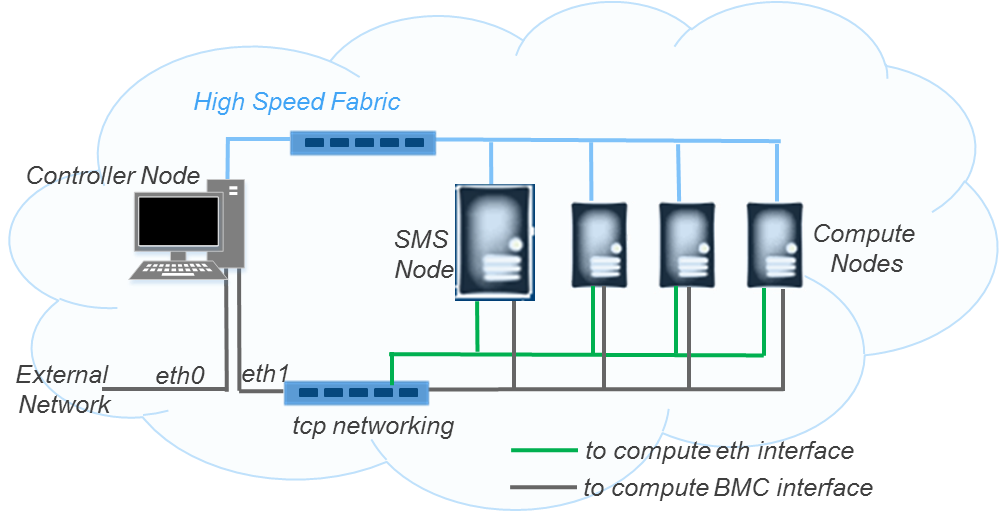
\includegraphics[width=0.85\linewidth]{HPCaaS-diagram.png}
\vspace*{-0.2cm}
\caption{Overview of physical cluster architecture.} \label{fig:physical_arch}
\end{figure}
\mbox{}

\vspace*{0.5cm}

An outline of the physical architecture discussed is shown in
Figure~\ref{fig:physical_arch} and highlights the high-level networking
configuration. The {\em master} host requires at least two Ethernet interfaces
with {\em eth0} connected to the local data center network and {\em eth1} used
to provision and manage the cluster backend (note that these interface names
are examples and may be different depending on local settings and OS
conventions). Two logical IP interfaces are expected to each compute node: the
first is the standard Ethernet interface that will be used for provisioning and
resource management. The second is used to connect to each host's BMC and is
used for power management and remote console access. Physical connectivity for
these two logical IP networks is often accommodated via separate cabling and
switching infrastructure; however, an alternate configuration can also be
accommodated via the use of a shared NIC, which runs a packet filter to divert
management packets between the host and BMC.

 In addition to the IP networking, there is a high-speed network
(\InfiniBand{} in this recipe) that is also connected to each of the
hosts. This high speed network is used for application message passing and
optionally for \Lustre{} connectivity as well.

NOTE: This recipe sets various environment variables in one section and use them 
in other section. So users are expected to use single shell session for successful 
execution of this recipe. Appendix A provides reference to prebuilt recipe, and 
useful for users who wants to try out with minimum human interactions.


% -*- mode: latex; fill-column: 120; -*- 

\subsection{Inputs} \label{sec:inputs}
As this recipe details installing a cluster starting from bare-metal, there is a requirement to define IP addresses and
gather hardware MAC addresses in order to support a controlled provisioning process. These values are necessarily unique
to the hardware being used, and this document uses variable substitution (\texttt{\$\{variable\}}) in the command-line
examples that follow to highlight where local site inputs are required. A summary of the required and optional variables
used throughout this recipe are presented below. Note that while the example definitions above correspond to a small
4-node compute subsystem, the compute parameters are defined in array format to accommodate logical extension to larger
node counts. \\

\vspace*{0.2cm}
\begin{tabular}{@{}>{\textbullet}l p{7cm} l}
& \texttt{\$\{sms\_name\}} & {\small \# Hostname for SMS server} \\
& \texttt{\$\{sms\_ip\}} & {\small \# Internal IP address on SMS server}  \\
& \texttt{\$\{sms\_eth\_internal\}} & {\small \# Internal Ethernet interface on SMS} \\
& \texttt{\$\{eth\_provision\}} & {\small \# Provisioning interface for computes} \\
& \texttt{\$\{internal\_netmask\}} & {\small \# Subnet netmask for internal network} \\
& \texttt{\$\{ntp\_server\}} & {\small \# Local ntp server for time synchronization} \\
& \texttt{\$\{bmc\_username\}} & {\small \# BMC username for use by IPMI} \\
& \texttt{\$\{bmc\_password\}} & {\small \# BMC password for use by IPMI} \\
& \texttt{\$\{num\_computes\}} & {\small \# Total \# of desired compute nodes} \\
& \texttt{\$\{c\_ip[0]\}}, \, \texttt{\$\{c\_ip[1]\}}, ... & {\small \# Desired compute node addresses} \\
& \texttt{\$\{c\_bmc[0]\}}, \texttt{\$\{c\_bmc[1]\}}, ... & {\small \# BMC addresses for computes} \\
& \texttt{\$\{c\_mac[0]\}}, \texttt{\$\{c\_mac[1]\}}, ... & {\small \# MAC addresses for computes} \\
& \texttt{\$\{compute\_regex\}} & {\small \# Regex matching all compute node names (e.g. ``c*'')} \\
& \texttt{\$\{compute\_prefix\}} & {\small \# Prefix for compute node names (e.g. ``c'')} \\
\end{tabular}

\vspace*{0.2cm}
\noindent {Optional:} 
\vspace*{0.1cm}

\begin{tabular}{@{}>{\textbullet}l p{7cm} l}
& \texttt{\$\{mgs\_fs\_name\}} & {\small \# Lustre MGS mount name} \\
& \texttt{\$\{sms\_ipoib\}} & {\small \# IPoIB address for SMS server} \\
& \texttt{\$\{ipoib\_netmask\}} & {\small \# Subnet netmask for internal IPoIB} \\
& \texttt{\$\{c\_ipoib[0]\}}, \texttt{\$\{c\_ipoib[1]\}}, ... & {\small \# IPoIB addresses for computes} \\
& \texttt{\$\{kargs\}} & {\small \# Kernel boot arguments} \\  
\end{tabular}

\begin{server_config}
///////Stoppping pomt ////////

ohpc_pkg="${ohpc_pkg:-https://github.com/openhpc/ohpc/releases/download/v1.1.GA/ohpc-release-centos7.2-1.1-1.x86_64.rpm}"
nodename_prefix="${nodename_prefix:-c}"
chpc_base=”ohpc”
hpc_slurm_partition=normal
# Prefix for compute node hostnames
cnodename_prefix= "${cnodename_prefix:-cc}"
# Local (internal) hostname on SMS
controller_name="${controller_name=sun-hn3}"
# Local (internal) IP address on SMS
controller_ip="${controller_ip=192.168.46.13}"
# cloud subnet CIDR
cc_subnet_cidr="${cc_subnet_cidr=192.168.46.0/24}"
# cloud subnet DHCP range
cc_subnet_dhcp_start="${cc_subnet_dhcp_start=192.168.46.130}"
cc_subnet_dhcp_end="${cc_subnet_dhcp_end=192.168.46.135}"
sms_mac=a4:bf:01:0c:e1:42
sms_bmc=192.168.46.58
# BMC user credentials for use by IPMI
sms_bmc_username="${sms_bmc_username:-root}"
sms_bmc_password="${sms_bmc_password:-root}"
cloud compute node characterstics (aka nova flavor)
SMS_RAM_MB=24456
SMS_CPU=16
\end{server_config}


% Bare Metal Node Operating System --------------------------------------------
\clearpage
% ohpc_validation_comment  #   XFILEX chpc_prepare_image
\section{Preparing Bare Metal Node Operating System}\label{sec:baremetalprep}


   This guide uses diskimage-builder utility to build and configure OS images 
for the sms (controller) node as well as compute nodes.  Preparing images is 
an optional part of the overall recipe. If user has predefined images, then 
environment variable "chpc\_create\_new\_image" must be reset and 
path to images must be provided using environment variable "chpc\_image\_deploy\_kernel", "chpc\_image\_deploy\_ramdisk",
"chpc\_image\_user", and "chpc\_image\_sms". 

In this example cloud images are built on controller node ("[ctrlr]\# "). Once images are built, they are stored in the standard openHPC Path.
In this recipe we will create utility functions for each functionality and then integrate them to make a complete receipe to create a compute node OS image. First setup a path for images to be stored.

% begin_ohpc_run
% ohpc_validation_newline
% ohpc_validation_comment #   XFILEX chpc_prepare_image
%% ohpc_validation_comment # SECTION BMNOS 
% ohpc_validation_comment Set cloud image path 
% ohpc_validation_comment 
\begin{lstlisting}[language=bash,keywords={},upquote=true]
[ctrlr](*\#*) CHPC_CLOUD_IMAGE_PATH=/opt/ohpc/admin/images/cloud/
\end{lstlisting}
% end_ohpc_run




\subsection{Install and Setup diskimage-builder}\label{sec:dib_install}

	Images can be built on any supported OS. In this example we will install and build images on controller node, user can do same on a system independent of their production cluster. We will create common functions to install diskimage-builder and its dependencies from base OS distro.

	Create a function to install diskimage-builder

% begin_ohpc_run
% ohpc_validation_newline
%% ohpc_validation_comment # SECTION BMNOS
% ohpc_validation_comment function to install diskimage-builder
% ohpc_validation_comment
\begin{lstlisting}[language=bash,keywords={}]
[ctrlr](*\#*) function setup_dib() {
\end{lstlisting}
% end_ohpc_run
	Install diskimage-builder and its dependencies
% begin_ohpc_run
%% ohpc_validation_comment # SECTION BMNOS
% ohpc_validation_comment   Install diskimage-builder 
% ohpc_validation_comment
\begin{lstlisting}[language=bash,keywords={}]
[ctrlr](*\#*)     yum -y install diskimage-builder PyYAML

\end{lstlisting}
% end_ohpc_run

% begin_ohpc_run
%% ohpc_validation_comment # SECTION BMNOS
% ohpc_validation_comment   Install grub dependency 
% ohpc_validation_comment
\begin{lstlisting}[language=bash,keywords={}]
[ctrlr](*\#*)     yum -y install parted
\end{lstlisting}
% end_ohpc_run

	diskimage-builder installed from the base repository does not have a group install feature. So add our patch (Note: this probably will be included into RPM and will be part of that rpm installation)

% begin_ohpc_run
%% ohpc_validation_comment # SECTION BMNOS
% ohpc_validation_comment   Fix for group install
% ohpc_validation_comment

\begin{lstlisting}[language=bash,keywords={}]
[ctrlr](*\#*)     yum -y localinstall /tmp/dib*
[ctrlr](*\#*) } # end of function
\end{lstlisting}
% end_ohpc_run


\newpage
\subsection{Setup common environment for diskimage-builder}\label{sec:dib_environment}
diskimage-builder or dib uses environment variables and elements to customize the images. For debugging purpose, we will create default user chpc with a password intel8086, with sudo privilege. These variables are used by element devuser. 

\begin{lstlisting}[language=bash,keywords={}]
[ctrlr](*\#*) export DIB_DEV_USER_USERNAME=chpc
[ctrlr](*\#*) export DIB_DEV_USER_PASSWORD=intel8086
[ctrlr](*\#*) export DIB_DEV_USER_PWDLESS_SUDO=1
\end{lstlisting}

Now add path to custom elements which are not part of base diskimage-builder. OpenHPC provides few HPC elements. [Note: This also can be part of openHPC provided rpm for dib. In that case remove this step]

\begin{lstlisting}[language=bash,keywords={}]
[ctrlr](*\#*) export ELEMENTS_PATH="$(realpath ../../dib/hpc/elements)"
\end{lstlisting}

Add path to HPC specific files [note: same as earlier, this too can be part of rpm package]

\begin{lstlisting}[language=bash,keywords={}]
[ctrlr](*\#*) export DIB_HPC_FILE_PATH="$(realpath ../../dib/hpc/hpc-files/)"
\end{lstlisting}

HPC elements are common for OpenHPC and Intel HPC Orchestrator, environment variable "DIB\_HPC\_BASE" tell dib which one to pick. For OpenHPC set environment variable


\begin{lstlisting}[language=bash,keywords={}]
[ctrlr](*\#*) export DIB_ HPC_BASE="ohpc"
\end{lstlisting}

Make sure open hpc packages is installed. ohpc\_pkg is one of the input setup earlier in this document.

\begin{lstlisting}[language=bash,keywords={}]
[ctrlr](*\#*) yum -y install ${ohpc_pkg}
\end{lstlisting}

Export same to DIB.

\begin{lstlisting}[language=bash,keywords={}]
[ctrlr](*\#*) export DIB_HPC_OHPC_PKG=${ohpc_pkg}
\end{lstlisting}

Create list of HPC elements needed to build HPC images, by starting hpc-env-base. This element will setup basic hpc environment to build hpc images.

\begin{lstlisting}[language=bash,keywords={}]
[ctrlr](*\#*) DIB_HPC_ELEMENTS="hpc-env-base"
\end{lstlisting}

\newpage
\subsection{Preparing ironic deploy images}\label{sec:ironic_deploy_images}
	Ironic uses deploy images (deploy\_kernel) to bootstrap the provisioning of user images.  This section will create a function to build deploy images. 

	Start by creating a function prepare\_deploy\_image

% begin_ohpc_run
% ohpc_validation_newline
% ohpc_validation_comment function to prepare deploy images
% ohpc_validation_comment
\begin{lstlisting}[language=bash,keywords={}]
[ctrlr](*\#*) function prepare_deploy_image() {
\end{lstlisting}
% end_ohpc_run 

	Check if user has requested to create images by verifying environment variables chpc\_create\_new\_image, chpc\_image\_deploy\_kernel and chpc\_image\_deploy\_ramdisk. If user already supplied images then we will copy images to our common image location and setup environment variable for later use.

% begin_ohpc_run
\begin{lstlisting}[language=bash,keywords={}]
[ctrlr](*\#*)    if [[ ${chpc_create_new_image} -ne 1 ]] && [[ -s $chpc_image_deploy_kernel ]] && [[ -s $chpc_image_deploy_ramdisk ]]; then
[ctrlr](*\#*)        # need to create an image, image is provided by user
[ctrlr](*\#*)        echo "Skiping cloud deploy-image build, Image provided:"
[ctrlr](*\#*)        echo "Deploy ramdisk Image:$chpc_image_deploy_ramdisk"
[ctrlr](*\#*)        # Store Images file
[ctrlr](*\#*)        CHPC_IMAGE_DEST=$CHPC_CLOUD_IMAGE_PATH/$(basename $chpc_image_deploy_kernel)
[ctrlr](*\#*)           if [[ ! -e $CHPC_IMAGE_DEST ]]; then
[ctrlr](*\#*)           sudo cp -f $chpc_image_deploy_kernel $CHPC_CLOUD_IMAGE_PATH/
[ctrlr](*\#*)        fi
[ctrlr](*\#*)        chpc_image_deploy_kernel=$CHPC_IMAGE_DEST
[ctrlr](*\#*)        CHPC_IMAGE_DEST=$CHPC_CLOUD_IMAGE_PATH/$(basename $chpc_image_deploy_ramdisk)
[ctrlr](*\#*)        if [[ ! -e $CHPC_IMAGE_DEST ]]; then
[ctrlr](*\#*)           sudo cp -f $chpc_image_deploy_ramdisk $CHPC_CLOUD_IMAGE_PATH/
[ctrlr](*\#*)        fi
[ctrlr](*\#*)        chpc_image_deploy_ramdisk=$CHPC_IMAGE_DEST
[ctrlr](*\#*)    else
[ctrlr](*\#*)        echo "Building new Cloud Deploy Image"
[ctrlr](*\#*)        echo "====================================================================="
[ctrlr](*\#*)        echo "=== Preparing cloud-hpc deploy images for ironic====================="
[ctrlr](*\#*)        echo "====================================================================="
[ctrlr](*\#*)        # prepare deploy images
[ctrlr](*\#*)        # Install dib if it is not already installed
[ctrlr](*\#*)        setup_dib
[ctrlr](*\#*)        # Unset any previos envirnment flag
[ctrlr](*\#*)        unset DIB_YUM_REPO_CONF   
[ctrlr](*\#*)        #  Install git if it is not already installed
[ctrlr](*\#*)        yum -y install git
[ctrlr](*\#*)        # make sure to get ironic component from stable mitaka release
[ctrlr](*\#*)        export DIB_REPOREF_ironic_agent=stable/mitaka
[ctrlr](*\#*)        disk-image-create ironic-agent centos7 -o icloud-hpc-deploy-c7
[ctrlr](*\#*)        echo "====================================================================="
[ctrlr](*\#*)        echo "=== cloud-hpc deploy images Complete ================================"
[ctrlr](*\#*)        echo "====================================================================="
[ctrlr](*\#*)        chpc_image_deploy_kernel="$( realpath icloud-hpc-deploy-c7.kernel)"
[ctrlr](*\#*)        chpc_image_deploy_ramdisk="$( realpath icloud-hpc-deploy-c7.initramfs)"
[ctrlr](*\#*)        # Store Images file
[ctrlr](*\#*)        mkdir -p $CHPC_CLOUD_IMAGE_PATH/
[ctrlr](*\#*)        sudo mv -f $chpc_image_deploy_kernel $CHPC_CLOUD_IMAGE_PATH/
[ctrlr](*\#*)        chpc_image_deploy_kernel=$CHPC_CLOUD_IMAGE_PATH/$(basename $chpc_image_deploy_kernel)
[ctrlr](*\#*)        sudo mv -f $chpc_image_deploy_ramdisk $CHPC_CLOUD_IMAGE_PATH/
[ctrlr](*\#*)        chpc_image_deploy_ramdisk=$CHPC_CLOUD_IMAGE_PATH/$(basename $chpc_image_deploy_ramdisk)
[ctrlr](*\#*)     fi
[ctrlr](*\#*) } # end of function
\end{lstlisting}

% end_ohpc_run 





\newpage
\subsection{Preparing user images for bare metal instances}\label{sec:bare_metal_user_images}
For "HPC as a Service" we will building 2 user images (1 for sms node and 1 for compute node) and 2 deploy images. User images we build here will be customized with OpenHPC using HPC specific elements. 

\subsubsection{Preparing user image for head node OS}\label{sec:head_node_images}
%%	Building head node (SMS) images requires installing the server packages of HPC components into the image. This is accomplished by setting image type to sms. Default image type in hpc elements is "compute". We will create a function prepare\_sms\_image to build this image, which will be called later in document.

% begin_ohpc_run
% ohpc_validation_newline
% ohpc_validation_comment function to prepare head node
% ohpc_validation_comment
\begin{lstlisting}[language=bash,keywords={}]
[ctrlr](*\#*) function prepare_sms_image() {
\end{lstlisting} 
% end_ohpc_run

	Check if user has requested to create images by verifying environment variables chpc\_create\_new\_image and chpc\_image\_sms. If user already supplied images then we will copy images to our common image location and setup environment variable for later use.
	
% begin_ohpc_run
\begin{lstlisting}[language=bash,keywords={}]
[ctrlr](*\#*)     if [[ ${chpc_create_new_image} -ne 1 ]] && [[ -s $chpc_image_sms ]]; then
[ctrlr](*\#*)         # No need to create an image, image is provided by user
[ctrlr](*\#*)         echo -n "Skiping cloud sms-image build, Image provided:"
[ctrlr](*\#*)         echo "$chpc_image_sms"
[ctrlr](*\#*)         CHPC_IMAGE_DEST=$CHPC_CLOUD_IMAGE_PATH/$(basename $chpc_image_sms)
[ctrlr](*\#*)         if [[ ! -e $CHPC_IMAGE_DEST ]]; then
[ctrlr](*\#*)             sudo cp $chpc_image_sms $CHPC_CLOUD_IMAGE_PATH
[ctrlr](*\#*)         fi
[ctrlr](*\#*)         chpc_image_sms=$CHPC_IMAGE_DEST
[ctrlr](*\#*)     else
\end{lstlisting} 
% end_ohpc_run

	If user has not supplied images then we will build the sms image here. Disk-image-builder supports two types of HPC images, "sms" and "compute".  

% begin_ohpc_run
\begin{lstlisting}[language=bash,keywords={}]
[ctrlr](*\#*)         # setup environment varioable to indicate sms image type
[ctrlr](*\#*)         setup_dib_hpc_base
[ctrlr](*\#*)         export DIB_HPC_IMAGE_TYPE=sms
\end{lstlisting} 
% end_ohpc_run

	Enable SLURM resource manager for "head" node.

% begin_ohpc_run

\begin{lstlisting}[language=bash,keywords={}]
[ctrlr](*\#*)         DIB_HPC_ELEMENTS+=" hpc-slurm"
\end{lstlisting} 
 % end_ohpc_run

	Add optional OpenHPC components.

% begin_ohpc_run

\begin{lstlisting}[language=bash,keywords={}]
[ctrlr](*\#*)         if [[ ${enable_mrsh} -eq 1 ]];then
[ctrlr](*\#*)             DIB_HPC_ELEMENTS+=" hpc-mrsh"
[ctrlr](*\#*)         fi
\end{lstlisting} 
 % end_ohpc_run

	We will also setup an HPC development environment on the HPC head node. 

	Start by enabling gnu compiler on head node.

% begin_ohpc_run

\begin{lstlisting}[language=bash,keywords={}]
[ctrlr](*\#*)         export DIB_HPC_COMPILER="gnu"
\end{lstlisting} 
 % end_ohpc_run

	Enable openmpi \& mvapich2.

% begin_ohpc_run

\begin{lstlisting}[language=bash,keywords={}]
[ctrlr](*\#*)         export DIB_HPC_MPI="openmpi mvapich2"
\end{lstlisting} 
 % end_ohpc_run

	Enable performance tools.

% begin_ohpc_run

\begin{lstlisting}[language=bash,keywords={}]
[ctrlr](*\#*)         export DIB_HPC_PERF_TOOLS="perf-tools"
\end{lstlisting} 
 % end_ohpc_run

	Enable 3rd party libraries serial-libs, parallel-libs, io-libs, python-libs and runtimes.

% begin_ohpc_run

\begin{lstlisting}[language=bash,keywords={}]
[ctrlr](*\#*)         export DIB_HPC_3RD_LIBS="serial-libs parallel-libs io-libs python-libs runtimes"
\end{lstlisting} 
 % end_ohpc_run

	Add HPC development environment element to list of elements.

% begin_ohpc_run

\begin{lstlisting}[language=bash,keywords={}]
[ctrlr](*\#*)         DIB_HPC_ELEMENTS+=" hpc-dev-env"
\end{lstlisting} 
 % end_ohpc_run

	Now create an sms image with element local-config, dhcp-all-interfaces, devuser, selinux-permisive, and all HPC specific elements. Element local-config copies your local environment into image, which is the local users, their password and permissions. Element devuser will create a new user specified by environment variable "DIB\_DEV\_USER\_USERNAME". The image will be named  {\em  icloud-hpc-cent7-sms }.

% begin_ohpc_run

\begin{lstlisting}[language=bash,keywords={}]
[ctrlr](*\#*)         disk-image-create centos7 vm local-config dhcp-all-interfaces \
[ctrlr](*\#*)         	devuser selinux-permissive $DIB_HPC_ELEMENTS -o icloud-hpc-cent7-sms
\end{lstlisting} 
 % end_ohpc_run

	It will take a while to build an image. Once the image is built, copy it to the standard OpenHPC path.

% begin_ohpc_run

\begin{lstlisting}[language=bash,keywords={}]
[ctrlr](*\#*)         chpc_image_sms="$( realpath icloud-hpc-cent7-sms.qcow2)"
[ctrlr](*\#*)         mkdir -p $CHPC_CLOUD_IMAGE_PATH
[ctrlr](*\#*)         mv -f $chpc_image_sms $CHPC_CLOUD_IMAGE_PATH
[ctrlr](*\#*)         chpc_image_sms=$CHPC_CLOUD_IMAGE_PATH/$(basename $chpc_image_sms)
[ctrlr](*\#*)     fi # end of else of or if
[ctrlr](*\#*) } # end of function
\end{lstlisting} 
 % end_ohpc_run

	Building head node (SMS) images requires installing the server packages of HPC components into the image. This is accomplished by setting the image type to "sms". The default image type in HPC elements is "compute". We will create a function prepare\_sms\_image to build this image, which will be called later in the document.

% begin_ohpc_run
% ohpc_validation_newline
% ohpc_validation_comment function to prepare head node
% ohpc_validation_comment
\begin{lstlisting}[language=bash,keywords={}]
[ctrlr](*\#*) function prepare_sms_image() {
\end{lstlisting} 
% end_ohpc_run

	Check if the user has requested to create images by verifying environment variables chpc\_create\_new\_image and chpc\_image\_sms. If the user has supplied images then we will copy images to our common image location and setup environment variables for later use.
	
% begin_ohpc_run
\begin{lstlisting}[language=bash,keywords={}]
[ctrlr](*\#*)     if [[ ${chpc_create_new_image} -ne 1 ]] && [[ -s $chpc_image_sms ]]; then
[ctrlr](*\#*)         # No need to create an image, image is provided by the user
[ctrlr](*\#*)         echo -n "Skipping cloud sms-image build, image provided:"
[ctrlr](*\#*)         echo "$chpc_image_sms"
[ctrlr](*\#*)         CHPC_IMAGE_DEST=$CHPC_CLOUD_IMAGE_PATH/$(basename $chpc_image_sms)
[ctrlr](*\#*)         if [[ ! -e $CHPC_IMAGE_DEST ]]; then
[ctrlr](*\#*)             sudo cp $chpc_image_sms $CHPC_CLOUD_IMAGE_PATH
[ctrlr](*\#*)         fi
[ctrlr](*\#*)         chpc_image_sms=$CHPC_IMAGE_DEST
[ctrlr](*\#*)     else
\end{lstlisting} 
% end_ohpc_run

	If the user has not supplied images then we will build the sms image here. Disk-image-builder supports two types of HPC images, "sms" and "compute".  

% begin_ohpc_run
\begin{lstlisting}[language=bash,keywords={}]
[ctrlr](*\#*)         # setup environment variable to indicate sms image type
[ctrlr](*\#*)         setup_dib_hpc_base
[ctrlr](*\#*)         export DIB_HPC_IMAGE_TYPE=sms
\end{lstlisting} 
% end_ohpc_run


	Enable the HPC resource manager into image. 

% begin_ohpc_run

\begin{lstlisting}[language=bash,keywords={}]
[ctrlr](*\#*)       DIB_HPC_ELEMENTS+=" hpc-pbs"
\end{lstlisting} 
 % end_ohpc_run

	Add optional OpenHPC components.

% begin_ohpc_run

\begin{lstlisting}[language=bash,keywords={}]
[ctrlr](*\#*)         if [[ ${enable_mrsh} -eq 1 ]];then
[ctrlr](*\#*)             DIB_HPC_ELEMENTS+=" hpc-mrsh"
[ctrlr](*\#*)         fi
\end{lstlisting} 
 % end_ohpc_run

	We will also setup an HPC development environment on the HPC head node. 

	Start by enabling the gnu compiler on head node.

% begin_ohpc_run

\begin{lstlisting}[language=bash,keywords={}]
[ctrlr](*\#*)         export DIB_HPC_COMPILER="gnu7"
\end{lstlisting} 
 % end_ohpc_run

	Enable openmpi \& mvapich2.

% begin_ohpc_run

\begin{lstlisting}[language=bash,keywords={}]
[ctrlr](*\#*)         export DIB_HPC_MPI="openmpi mvapich2"
\end{lstlisting} 
 % end_ohpc_run

	Enable performance tools.

% begin_ohpc_run

\begin{lstlisting}[language=bash,keywords={}]
[ctrlr](*\#*)         export DIB_HPC_PERF_TOOLS="perf-tools"
\end{lstlisting} 
 % end_ohpc_run

	Enable 3rd party libraries serial-libs, parallel-libs, io-libs, python-libs, and runtimes.

% begin_ohpc_run

\begin{lstlisting}[language=bash,keywords={}]
[ctrlr](*\#*)         export DIB_HPC_3RD_LIBS="serial-libs parallel-libs io-libs python-libs runtimes"
\end{lstlisting} 
 % end_ohpc_run

	Add the HPC development environment element to the list of elements.

% begin_ohpc_run

\begin{lstlisting}[language=bash,keywords={}]
[ctrlr](*\#*)         DIB_HPC_ELEMENTS+=" hpc-dev-env"
\end{lstlisting} 
 % end_ohpc_run

	Now create an sms image with the following elements: local-config, dhcp-all-interfaces, devuser, selinux-permisive, and all HPC specific elements. Element local-config copies your local environment into the image, which is the local users, their password, and permissions. Element devuser will create a new user specified by environment variable "DIB\_DEV\_USER\_USERNAME". The image will be named  {\em  icloud-hpc-cent7-sms}.

% begin_ohpc_run

\begin{lstlisting}[language=bash,keywords={}]
[ctrlr](*\#*)         disk-image-create centos7 vm local-config dhcp-all-interfaces \
[ctrlr](*\#*)         	devuser selinux-permissive $DIB_HPC_ELEMENTS -o icloud-hpc-cent7-sms
\end{lstlisting} 
 % end_ohpc_run

	It will take awhile to build an image. Once the image is built, copy it to the standard OpenHPC path.

% begin_ohpc_run

\begin{lstlisting}[language=bash,keywords={}]
[ctrlr](*\#*)         chpc_image_sms="$( realpath icloud-hpc-cent7-sms.qcow2)"
[ctrlr](*\#*)         mkdir -p $CHPC_CLOUD_IMAGE_PATH
[ctrlr](*\#*)         mv -f $chpc_image_sms $CHPC_CLOUD_IMAGE_PATH
[ctrlr](*\#*)         chpc_image_sms=$CHPC_CLOUD_IMAGE_PATH/$(basename $chpc_image_sms)
[ctrlr](*\#*)     fi # end of else of or if
[ctrlr](*\#*) } # end of function
\end{lstlisting} 
 % end_ohpc_run



\subsubsection{Preparing user image for compute node OS}\label{sec:compute_node_images}
%%	To build compute node images, we need to install the client packages of HPC components. This is accomplished by setting image type to compute. Default image type in HPC elements is "compute". We will then instruct disk-image-builder to install client HPC packages one by one. We will do all these in a shell function prepare\_user\_images.

% begin_ohpc_run
% ohpc_validation_newline
% ohpc_validation_comment function to prepare compute node
% ohpc_validation_comment
\begin{lstlisting}[language=bash,keywords={}]
[ctrlr](*\#*) function prepare_user_image() {

\end{lstlisting} 

	Check if user has already supplied compute node images by checking environment variables:
	
		 chpc\_create\_new\_image and chpc\_image\_user.
		  
	If image is supplied then we will copy image to ohpc image location and setup our environemnt variable to point to image location 
% begin_ohpc_run
\begin{lstlisting}[language=bash,keywords={}]
[ctrlr](*\#*)    if [[ ${chpc_create_new_image} -ne 1 ]] && [[ -s $chpc_image_user ]]; then
[ctrlr](*\#*)       # No need to create an image, image is provided by user
[ctrlr](*\#*)       echo -n "Skiping cloud user-image build, Image provided:"
[ctrlr](*\#*)       echo "$chpc_image_user"
[ctrlr](*\#*)       CHPC_IMAGE_DEST=$CHPC_CLOUD_IMAGE_PATH/$(basename $chpc_image_user)
[ctrlr](*\#*)       if [[ ! -e $CHPC_IMAGE_DEST ]]; then
[ctrlr](*\#*)          sudo cp $chpc_image_user $CHPC_CLOUD_IMAGE_PATH
[ctrlr](*\#*)       fi
[ctrlr](*\#*)       chpc_image_user=$CHPC_IMAGE_DEST
[ctrlr](*\#*)    else
[ctrlr](*\#*)    

\end{lstlisting} 

% end_ohpc_run

	Create a new image, if one is not supplied by a user. 	
	
	Set image type to compute  

% begin_ohpc_run
\begin{lstlisting}[language=bash,keywords={}]
[ctrlr](*\#*)       setup_dib_hpc_base
[ctrlr](*\#*)       export DIB_HPC_IMAGE_TYPE=compute
\end{lstlisting} 
% end_ohpc_run

	Enable SLURM resource manager for compute node.

% begin_ohpc_run

\begin{lstlisting}[language=bash,keywords={}]
[ctrlr](*\#*)       DIB_HPC_ELEMENTS+=" hpc-slurm"
\end{lstlisting} 
 % end_ohpc_run

	Add optional OpenHPC Components

% begin_ohpc_run

\begin{lstlisting}[language=bash,keywords={}]
[ctrlr](*\#*)       if [[ ${enable_mrsh} -eq 1 ]];then
[ctrlr](*\#*)           DIB_HPC_ELEMENTS+=" hpc-mrsh"
[ctrlr](*\#*)       fi
\end{lstlisting} 
 % end_ohpc_run

	Create a compute node image with element local-config, dhcp-all-interfaces, devuser, selinux-permisive and all hpc specific elements. Element local-config copies your local environment into image, which is the local users, their password and permissions. Element devuser will create new user specified by environment variable "DIB\_DEV\_USER\_USERNAME". We will name the image {\em  icloud-hpc-cent7 }

% begin_ohpc_run

\begin{lstlisting}[language=bash,keywords={}]
[ctrlr](*\#*)       disk-image-create centos7 vm local-config dhcp-all-interfaces \
[ctrlr](*\#*)         devuser selinux-permissive $DIB_HPC_ELEMENTS -o icloud-hpc-cent7
\end{lstlisting} 
 % end_ohpc_run 


	It will take a while to build an image. Once the image is built, copy it to standard OpenHPC path.

% begin_ohpc_run

\begin{lstlisting}[language=bash,keywords={}]
[ctrlr](*\#*)       chpc_image_user="$( realpath icloud-hpc-cent7.qcow2)"
[ctrlr](*\#*)       mkdir -p $CHPC_CLOUD_IMAGE_PATH
[ctrlr](*\#*)       mv -f $chpc_image_user $CHPC_CLOUD_IMAGE_PATH
[ctrlr](*\#*)       chpc_image_user=$CHPC_CLOUD_IMAGE_PATH/$(basename $chpc_image_user)
[ctrlr](*\#*)     fi # end of else of or if
[ctrlr](*\#*) } # end of function
\end{lstlisting} 
 % end_ohpc_run


	To build compute node images, we need to install the client packages of HPC components. This is accomplished by setting the image type to "compute". Note the default image type in HPC elements is "compute". We will then instruct disk-image-builder to install client HPC packages one by one. All of these action will be completed in the shell function prepare\_user\_images.

% begin_ohpc_run
% ohpc_validation_newline
% ohpc_validation_comment function to prepare compute node
% ohpc_validation_comment
\begin{lstlisting}[language=bash,keywords={}]
[ctrlr](*\#*) function prepare_user_image() {

\end{lstlisting} 

	Check if the user has already supplied compute node images by checking the environment variables:
	
		 chpc\_create\_new\_image and chpc\_image\_user.
		  
	If the image is supplied then we will copy that image to the OHPC image location and setup our environemnt variable to point to the image location.
% begin_ohpc_run
\begin{lstlisting}[language=bash,keywords={}]
[ctrlr](*\#*)    if [[ ${chpc_create_new_image} -ne 1 ]] && [[ -s $chpc_image_user ]]; then
[ctrlr](*\#*)       # No need to create an image, image is provided by the user
[ctrlr](*\#*)       echo -n "Skipping cloud user-image build, image provided:"
[ctrlr](*\#*)       echo "$chpc_image_user"
[ctrlr](*\#*)       CHPC_IMAGE_DEST=$CHPC_CLOUD_IMAGE_PATH/$(basename $chpc_image_user)
[ctrlr](*\#*)       if [[ ! -e $CHPC_IMAGE_DEST ]]; then
[ctrlr](*\#*)          sudo cp $chpc_image_user $CHPC_CLOUD_IMAGE_PATH
[ctrlr](*\#*)       fi
[ctrlr](*\#*)       chpc_image_user=$CHPC_IMAGE_DEST
[ctrlr](*\#*)    else
[ctrlr](*\#*)    

\end{lstlisting} 

% end_ohpc_run

	Create a new image, if one is not supplied by a user. 	
	
	Set image type to "compute".

% begin_ohpc_run
\begin{lstlisting}[language=bash,keywords={}]
[ctrlr](*\#*)       setup_dib_hpc_base
[ctrlr](*\#*)       export DIB_HPC_IMAGE_TYPE=compute
\end{lstlisting} 
% end_ohpc_run


	Enable the HPC resource manager into image. 

% begin_ohpc_run

\begin{lstlisting}[language=bash,keywords={}]
[ctrlr](*\#*)       DIB_HPC_ELEMENTS+=" hpc-pbs"
\end{lstlisting} 
 % end_ohpc_run



	Add optional OpenHPC components.

% begin_ohpc_run

\begin{lstlisting}[language=bash,keywords={}]
[ctrlr](*\#*)       if [[ ${enable_mrsh} -eq 1 ]];then
[ctrlr](*\#*)           DIB_HPC_ELEMENTS+=" hpc-mrsh"
[ctrlr](*\#*)       fi
\end{lstlisting} 
 % end_ohpc_run

	Create a compute node image with the following elements: local-config, dhcp-all-interfaces, devuser, selinux-permissive and all HPC specific elements. Element local-config copies your local environment into the image, which is the local users, their password, and permissions. Element devuser will create a new user specified by the environment variable "DIB\_DEV\_USER\_USERNAME". We will name the image {\em  icloud-hpc-cent7 }

% begin_ohpc_run

\begin{lstlisting}[language=bash,keywords={}]
[ctrlr](*\#*)       disk-image-create centos7 vm local-config dhcp-all-interfaces \
[ctrlr](*\#*)         devuser selinux-permissive $DIB_HPC_ELEMENTS -o icloud-hpc-cent7
\end{lstlisting} 
 % end_ohpc_run 


	It will take awhile to build an image. Once the image is built, copy it to the standard OpenHPC path.

% begin_ohpc_run

\begin{lstlisting}[language=bash,keywords={}]
[ctrlr](*\#*)       chpc_image_user="$( realpath icloud-hpc-cent7.qcow2)"
[ctrlr](*\#*)       mkdir -p $CHPC_CLOUD_IMAGE_PATH
[ctrlr](*\#*)       mv -f $chpc_image_user $CHPC_CLOUD_IMAGE_PATH
[ctrlr](*\#*)       chpc_image_user=$CHPC_CLOUD_IMAGE_PATH/$(basename $chpc_image_user)
[ctrlr](*\#*)     fi # end of else of or if
[ctrlr](*\#*) } # end of function
\end{lstlisting} 
 % end_ohpc_run



\newpage
\subsubsection{Putting it all together }\label{sec:compute_node_images_all_together}
	We created a helper function. Call these functions in order to generate images for compute node.

% begin_ohpc_run
% ohpc_validation_newline
%% ohpc_validation_comment #   XFILEX chpc_prepare_image
% ohpc_validation_comment Build HPC user image
% ohpc_validation_comment 
%% Next line will only appear in documentation

	Add these print banners to start image building for your scripting to help know where they are in the install.

\begin{lstlisting}[language=bash,keywords={},upquote=true]
[ctrlr](*\#*) echo "########################################################################"
[ctrlr](*\#*) echo "########################### Starting SMS Image   ###########################"
[ctrlr](*\#*) echo "########################################################################"
\end{lstlisting}
%% Next line will only appear in documentation

	Prepare image for sms node by calling function prepare\_image\_sms

\begin{lstlisting}[language=bash,keywords={},upquote=true]
[ctrlr](*\#*) prepare\_sms\_image
\end{lstlisting}

%% Next line will only appear in documentation

	Print banner to indicate end of image creation

\begin{lstlisting}[language=bash,keywords={},upquote=true]
[ctrlr](*\#*) echo $chpc_image_sms
[ctrlr](*\#*) echo "########################################################################"
[ctrlr](*\#*) echo "########################### sms image is done ##########################"
[ctrlr](*\#*) echo "########################################################################"
\end{lstlisting}
%% Next line will only appear in documentation
	Prepare image for compute node by calling function prepare\_user\_image

\begin{lstlisting}[language=bash,keywords={},upquote=true]
[ctrlr](*\#*) prepare\_user\_image
\end{lstlisting}

%% Next line will only appear in documentation
	Print banner to indicate end of user creation
	
\begin{lstlisting}[language=bash,keywords={},upquote=true]
[ctrlr](*\#*) echo $chpc_image_user
[ctrlr](*\#*) echo "########################################################################"
[ctrlr](*\#*) echo "########################## user image is done ##########################"
[ctrlr](*\#*) echo "########################################################################"
\end{lstlisting}

%% Next line will only appear in documentation
	
	Prepare deploye images for ironic provisioning 

\begin{lstlisting}[language=bash,keywords={},upquote=true]
[ctrlr](*\#*) prepare\_deploy\_image
\end{lstlisting}

%% Next line will only appear in documentation
	
	Print banner to indicate end of user creation

\begin{lstlisting}[language=bash,keywords={},upquote=true]
[ctrlr](*\#*) echo $chpc_image_deploy_kernel
[ctrlr](*\#*) echo $chpc_image_deploy_ramdisk
[ctrlr](*\#*) echo "########################################################################"
[ctrlr](*\#*) echo "######################### deploy image is done #########################"
[ctrlr](*\#*) echo "########################################################################"
\end{lstlisting}
% end_ohpc_run




%%\subsection{Introduction to diskimage-builder}\label{sec:din_intro}
%%It is a utility to build and configure OS images for sms node as well compute node. It uses prebuild minimum OS images from base distro, which it further customizes as per user request. Diskimage-builder is a framework which uses many elements (similar to plug-ins) to customize the image. Base distribution of diskimage-builder comes with pre-defined elements. This recipe uses additional HPC elements which were built to customize images based on OpenHPC components.

\subsubsection{HPC Elements to build OpenHPC Images}

"HPC as a service" uses 4 HPC specific elements in addition to pre-packaged elements comes with diskimage-builder.

hpc-dev-env: 
	This is mainly used to create sms images to create HPC development environment. It creates hpc development environment by installing following OpenHPC components within image: 
		ohpc-autotools, valgrind-ohpc, easybuild-ohpc, spack-ohpc, r\_base-ohpc
		mpi and compiler for chosen MPI and compiler via environment variable, \$DIB\_HPC\_COMPILER, \$DIB\_HPC\_MPI
		Performance Tools lmod-default with their 3rd party libraries.

hpc-env-base: TBC

hpc-mrsh:TBC

hpc-slurm: TBC

\subsubsection{Editing HPC Elements}

	TBC



% ------------------------------------------------------------------
\clearpage

\section{Preparing Cloud-Init} \label{sec:cloud-init_prep}
	OpenStack uses cloud-init for boot time initialization of cloud instances. This recipe relies on cloud-init to initialize HPC instances in an OpenStack cloud. This recipe prepares the cloud-init initialization template script, which is then updated with sms-ip and other environment variables just before the provisioning. This is than fed as user data to Nova during instance creation. Script generated here will be executed by root during bootup. 
The cloud-init templates are provided as a part "docs-chpc" RPM and installed at {\em /opt/ohpc/pub/doc/recipes/centos7/x86\_64/openstack/slurm/cloud\_hpc\_init/ohpc}. Here we will create similar tempalte and store into this same path. 



\subsection{Preparing template for compute node cloud-init} \label{sec:c_i-template_compute_node}
	Create an empty chpc\_init file and open for editing. You can also use  existing template and modify.

	Start editing by adding some environment variable, first one is to set path to shared folder for cloud-init

% begin_ohpc_run
% ohpc_validation_newline
% ohpc_validation_comment #   XFILEX
% ohpc_validation_comment #   PFILEP
% ohpc_command #!/bin/bash
% ohpc_validation_comment #   FILE: chpc_init

\begin{lstlisting}[language=bash,keywords={}]
[ctrlr](*\#*) chpcInitPath=/opt/ohpc/admin/cloud_hpc_init
[ctrlr](*\#*) SCRIPTDIR="$( cd "$( dirname "$( readlink -f "${BASH_SOURCE[0]}" )" )" && pwd -P && echo x)"
[ctrlr](*\#*) SCRIPTDIR="${SCRIPTDIR%x}"
[ctrlr](*\#*) cd $SCRIPTDIR
[ctrlr](*\#*) chpcInitPath=/opt/ohpc/admin/cloud_hpc_init

[ctrlr](*\#*) logger "chpcInit: Updating Compute Node with HPC configuration"
\end{lstlisting}
% end_ohpc_run

	Update rsyslog configuration file to send all the syslog to sms. sms\_ip is the tag used here is updated with IP of SMS node just before provisioning.

% begin_ohpc_run
% ohpc_validation_newline
\begin{lstlisting}[language=bash,keywords={}]
[ctrlr](*\#*) # Update rsyslog
[ctrlr](*\#*) cat /etc/rsyslog.conf | grep "<sms_ip>:514"
[ctrlr](*\#*) rsyslog_set=$?
[ctrlr](*\#*) if [ "${rsyslog_set}" -ne "0" ]; then
[ctrlr](*\#*)    echo "*.* @<sms_ip>:514" >> /etc/rsyslog.conf
[ctrlr](*\#*) fi
[ctrlr](*\#*)  systemctl restart rsyslog
[ctrlr](*\#*) logger "chpcInit: rsyslog configuration complete, updating remaining HPC configuration"
\end{lstlisting}
% end_ohpc_run

	Assuming sms node nfs share /home, /opt/ohpc/pub, =/opt/ohpc/admin/cloud\_hpc\_init lets mount them during boot

% begin_ohpc_run
% ohpc_validation_newline
\begin{lstlisting}[language=bash,keywords={}]
[ctrlr](*\#*) # nfs mount directory from SMS head node to Compute Node
[ctrlr](*\#*) cat /etc/fstab | grep "<sms_ip>:/home"
[ctrlr](*\#*) home_exists=$?
[ctrlr](*\#*) if [ "${home_exists}" -ne "0" ]; then
[ctrlr](*\#*)     echo "<sms_ip>:/home /home nfs nfsvers=3,rsize=1024,wsize=1024,cto 0 0" >> /etc/fstab
[ctrlr](*\#*) fi
[ctrlr](*\#*) cat /etc/fstab | grep "<sms_ip>:/opt/ohpc/pub"
[ctrlr](*\#*) ohpc_pub_exists=$?
[ctrlr](*\#*) 
[ctrlr](*\#*) if [ "${ohpc_pub_exists}" -ne "0" ]; then
[ctrlr](*\#*)     echo "<sms_ip>:/opt/ohpc/pub /opt/ohpc/pub nfs nfsvers=3 0 0" >> /etc/fstab
[ctrlr](*\#*)     # Make sure we have directory to mount
[ctrlr](*\#*)     # Clean up if required
[ctrlr](*\#*)     if [ -e /opt/ohpc/pub ]; then
[ctrlr](*\#*)         echo "chpcInit: [WARNING] /opt/ohpc/pub already exists!!"
[ctrlr](*\#*)     fi
[ctrlr](*\#*) fi
[ctrlr](*\#*) mkdir -p /opt/ohpc/pub
[ctrlr](*\#*) mount /home
[ctrlr](*\#*) mount /opt/ohpc/pub
[ctrlr](*\#*) 
[ctrlr](*\#*) # Mount cloud_hpc_init
[ctrlr](*\#*) cat /etc/fstab | grep "sms_ip:$chpcInitPath"
[ctrlr](*\#*) CloudHPCInit_exist=$?
[ctrlr](*\#*) if [ "${CloudHPCInit_exist}" -ne "0" ]; then
[ctrlr](*\#*)     echo "<sms_ip>:$chpcInitPath $chpcInitPath nfs nfsvers=3 0 0" >> /etc/fstab
[ctrlr](*\#*) fi
[ctrlr](*\#*) mkdir -p $chpcInitPath
[ctrlr](*\#*) mount $chpcInitPath
[ctrlr](*\#*) # Restart nfs
[ctrlr](*\#*) systemctl restart nfs
[ctrlr](*\#*) 
\end{lstlisting}
% end_ohpc_run

	Have ntp sync with the sms node. 

% begin_ohpc_run
% ohpc_validation_newline

\begin{lstlisting}
[ctrlr](*\#*) # Restart ntp at CN
[ctrlr](*\#*) systemctl enable ntpd
[ctrlr](*\#*) # Update ntp server
[ctrlr](*\#*) cat /etc/ntp.conf | grep "server <sms_ip>"
[ctrlr](*\#*) ntp_server_exists=$?
[ctrlr](*\#*) if [ "${ntp_server_exists}" -ne "0" ]; then
[ctrlr](*\#*)     echo "server <sms_ip>" >> /etc/ntp.conf
[ctrlr](*\#*) fi
[ctrlr](*\#*) systemctl restart ntpd
[ctrlr](*\#*) # Sync time
[ctrlr](*\#*) ntpstat
[ctrlr](*\#*) #Sync sms node with compute nodes. sync users, slurm and enable munge by copying munge keys
[ctrlr](*\#*) # Sync following files to compute node
[ctrlr](*\#*) # Assuming nfs is setup properly
[ctrlr](*\#*) if [ -d $chpcInitPath ]; then
[ctrlr](*\#*)     # Update the slurm file
[ctrlr](*\#*)     cp -f -L $chpcInitPath/slurm.conf /etc/slurm/slurm.conf
[ctrlr](*\#*)     # Sync head node configuration with Compute Node
[ctrlr](*\#*)     cp -f -L $chpcInitPath/passwd /etc/passwd
[ctrlr](*\#*)     cp -f -L $chpcInitPath/group /etc/group
[ctrlr](*\#*)     cp -f -L $chpcInitPath/shadow /etc/shadow
[ctrlr](*\#*)     cp -f -L $chpcInitPath/authorized_keys /root/.ssh/
[ctrlr](*\#*)     cp -f -L $chpcInitPath/slurm.conf /etc/slurm/slurm.conf
[ctrlr](*\#*)     cp -f -L $chpcInitPath/slurm /etc/pam.d/slurm
[ctrlr](*\#*)     cp -f -L $chpcInitPath/munge.key /etc/munge/munge.key
[ctrlr](*\#*)     # For hostname resolution
[ctrlr](*\#*)     cp -f -L $chpcInitPath/hosts /etc/hosts
[ctrlr](*\#*)     # make sure that hostname mentioned into /etc/hosts matches machine hostname. TBD
[ctrlr](*\#*)     # Start slurm and munge 
[ctrlr](*\#*)     systemctl enable munge
[ctrlr](*\#*)     systemctl restart munge
[ctrlr](*\#*)     systemctl enable slurmd
[ctrlr](*\#*)     systemctl restart slurmd
[ctrlr](*\#*) else
[ctrlr](*\#*)     logger "chpcInit:ERROR: cannot stat nfs shared /opt directory, cannot copy HPC system files"
[ctrlr](*\#*) fi
\end{lstlisting}
% end_ohpc_run

	Update the hostname as per the sms node.

% begin_ohpc_run
% ohpc_validation_newline

\begin{lstlisting}[language=bash,keywords={}]
[ctrlr](*\#*) # Setup hostname as per the head node
[ctrlr](*\#*) #Find the hostname of this machine from the copied over /etc/hosts file
[ctrlr](*\#*) cc_ipaddrs=(`hostname -I`)
[ctrlr](*\#*) for cc_ipaddr in ${cc_ipaddrs[@]}; do
[ctrlr](*\#*)     cat /etc/hosts | grep ${cc_ipaddr} > /dev/null
[ctrlr](*\#*)     result=$?
[ctrlr](*\#*)     if [ "$result" -eq "0" ]; then
[ctrlr](*\#*)         cc_hostname=`cat /etc/hosts | grep ${cc_ipaddr} | cut -d$'\t' -f2`
[ctrlr](*\#*)         break
[ctrlr](*\#*)     fi
[ctrlr](*\#*) done
[ctrlr](*\#*) 
[ctrlr](*\#*) if [ -z "${cc_hostname}" ]; then
[ctrlr](*\#*)     logger "chpcInit:ERROR: No resolved hostname found for any IP address in /etc/hosts"
[ctrlr](*\#*)     exit 1
[ctrlr](*\#*) fi
[ctrlr](*\#*) 
[ctrlr](*\#*) #set the hostname
[ctrlr](*\#*) if [ $(hostname) != ${cc_hostname} ]; then
[ctrlr](*\#*)     hostnamectl set-hostname ${cc_hostname}
[ctrlr](*\#*) fi
\end{lstlisting}
% end_ohpc_run

	At this point, all pre-requisites for slurm should be met. Let's start the slurm daemon.

% begin_ohpc_run
% ohpc_validation_newline

\begin{lstlisting}[language=bash,keywords={}]
[ctrlr](*\#*) # Start slurm and munge 
[ctrlr](*\#*) systemctl enable munge
[ctrlr](*\#*) systemctl restart munge
[ctrlr](*\#*) systemctl enable slurmd
[ctrlr](*\#*) systemctl restart slurmd
\end{lstlisting}
%end_ohpc_run

	One last step to make sure ssh is working and enabled on compute nodes. Update/verify the permissions of ssh.

% begin_ohpc_run
% ohpc_validation_newline

\begin{lstlisting}[language=bash,keywords={}]
[ctrlr](*\#*) #Change file permissions in /etc/ssh to fix ssh into compute node
[ctrlr](*\#*) chmod 0600 /etc/ssh/ssh_host_*_key
\end{lstlisting}
% end_ohpc_run

	Save the file with name chpc\_init, we will use this file during baremetal node instance creation.


     Enable pbs Resource Manager on compute nodes.

% begin_ohpc_run
% ohpc_validation_newline

\begin{lstlisting}
[ctrlr](*\#*) #Sync sms node with compute nodes. sync users, HPC resource manager and enable munge by copying munge keys
[ctrlr](*\#*) # Sync following files to compute node
[ctrlr](*\#*) # Assuming nfs is setup properly
[ctrlr](*\#*) if [ -d $chpcInitPath ]; then
[ctrlr](*\#*)     # Update the pbs file
[ctrlr](*\#*)     perl -pi -e "s/PBS_SERVER=\S+/PBS_SERVER=${sms_name}/" /etc/pbs.conf
[ctrlr](*\#*)     # make sure that hostname mentioned into /etc/hosts matches machine hostname. 
[ctrlr](*\#*)     # configure pbs
[ctrlr](*\#*)     /opt/pbs/libexec/pbs_habitat
[ctrlr](*\#*)     perl -pi -e "s/\$clienthost \S+/\$clienthost ${sms_name}/" /var/spool/pbs/mom_priv/config
[ctrlr](*\#*)     echo "\$usecp *:/home /home" >> /var/spool/pbs/mom_priv/config 

[ctrlr](*\#*) else
[ctrlr](*\#*)     logger "chpcInit:ERROR: cannot stat nfs shared /opt directory, cannot copy HPC system files"
[ctrlr](*\#*) fi
\end{lstlisting}
% end_ohpc_run

	At this point, all pre-requisites for HPC resource manager should be met. Let's start the daemon.

% begin_ohpc_run
% ohpc_validation_newline

\begin{lstlisting}[language=bash,keywords={}]
[ctrlr](*\#*) # Start pbs 
[ctrlr](*\#*) systemctl enable pbs
[ctrlr](*\#*) systemctl start pbs
[ctrlr](*\#*) logger "chpcInit: Resource Manager configuration Complete"
\end{lstlisting}
%end_ohpc_run

	Save the file with name 'chpc\_init', we will use  file during the creation of baremetal node instances.




\newpage
\subsection{Preparing template for sms node cloud-init} \label{sec:c_i-template-sms-node}
	The cloud-init script for the SMS node is different than the compute node. The SMS node, when instantiated within OpenStack, serves as head node for HPC-as-a-Service, and hosts all services as a SMS node in an independent HPC cluster. The resource manager runs on the SMS node. The SMS node also works as a NFS server and exports users’ home directories and common software to the compute nodes. For more detail on SMS node functionality please refer to OpenHPC documentation http://www.openhpc.community/downloads/.

	In this recipe, we will prepare a cloud-init template script for the SMS node, which then is updated with compute node IP, NTP server, and other environmental variables, just before provisioning. 

	Create an empty chpc\_init file and open it for editing. You can also modify the existing template. Start editing by adding environment variable, which will be updated later, just before provisioning.

% begin_ohpc_run
% ohpc_validation_newline
% ohpc_validation_comment #   PFILEP
% ohpc_command #!/bin/bash
% ohpc_validation_comment # FILE: chpc_sms_init


\begin{lstlisting}[language=bash,keywords={}]
[ctrlr](*\#*) #Ensure the executing shell is in the same directory as the script.
[ctrlr](*\#*) SCRIPTDIR="$( cd "$( dirname "$( readlink -f "${BASH_SOURCE[0]}" )" )" && pwd -P && echo x)"
[ctrlr](*\#*) SCRIPTDIR="${SCRIPTDIR%x}"
[ctrlr](*\#*) cd $SCRIPTDIR
[ctrlr](*\#*) # Get the compute node prefix and number of compute nodes
[ctrlr](*\#*) cnodename_prefix=<update_cnodename_prefix>
[ctrlr](*\#*) num_ccomputes=<update_num_ccomputes>
[ctrlr](*\#*) ntp_server=<update_ntp_server>
[ctrlr](*\#*) sms_name=<update_sms_name>
[ctrlr](*\#*) logger "chpcsmsInit: Entered chpcsmsInit"

\end{lstlisting} 
 % end_ohpc_run

	Now, setup "nfs" share for cloud-init and files you want to send to compute nodes.

% begin_ohpc_run
% ohpc_validation_newline

\begin{lstlisting}[language=bash,keywords={}]
[ctrlr](*\#*) # setup cloudinit directory
[ctrlr](*\#*) chpcInitPath=/opt/ohpc/admin/cloud_hpc_init
[ctrlr](*\#*) # create directory if it is not present
[ctrlr](*\#*) mkdir -p $chpcInitPath
[ctrlr](*\#*) chmod 700 $chpcInitPath
[ctrlr](*\#*) # Copy public ssh key to shared drive
[ctrlr](*\#*) _ssh_path=/root/.ssh
[ctrlr](*\#*) if [ ! -e "$_ssh_path/hpcasservice" ]; then
[ctrlr](*\#*) 
[ctrlr](*\#*) 	if [ ! -d "$_ssh_path" ]; then
[ctrlr](*\#*) 		install -d -m 700 $_ssh_path
[ctrlr](*\#*) 	fi
[ctrlr](*\#*) 	ssh-keygen -t dsa -f $_ssh_path/hpcasservice -N '' -C "HPC Cluster key" > /dev/null 2>&1
[ctrlr](*\#*) 	cat $_ssh_path/hpcasservice.pub >> $_ssh_path/authorized_keys
[ctrlr](*\#*) 	chmod 0600 $_ssh_path/authorized_keys
[ctrlr](*\#*) fi
[ctrlr](*\#*) 	#update config
[ctrlr](*\#*) if [ ! -e "$_ssh_path/config" ]; then
[ctrlr](*\#*) 	echo "Host *" > $_ssh_path/config
[ctrlr](*\#*) 	echo "    IdentityFile ~/.ssh/hpcasservice" >> $_ssh_path/config
[ctrlr](*\#*) 	echo "    StrictHostKeyChecking=no" >> $_ssh_path/config
[ctrlr](*\#*) fi
[ctrlr](*\#*) cp -fpr $_ssh_path/authorized_keys $chpcInitPath
[ctrlr](*\#*) #Change file permissions in /etc/ssh to fix ssh into sms nodes
[ctrlr](*\#*) chmod 0600 /etc/ssh/ssh_host_*_key

\end{lstlisting} 
 % end_ohpc_run

	Share "/home, "/opt/ohpc/pub", and "/opt/ohpc/admin/cloud\_hpc\_initi" over "nfs"

% begin_ohpc_run
% ohpc_validation_newline

\begin{lstlisting}[language=bash,keywords={}]
[ctrlr](*\#*) # export CloudInit Path to nfs share
[ctrlr](*\#*) cat /etc/exports | grep "$chpcInitPath"
[ctrlr](*\#*) chpcInitPath_exported=$?
[ctrlr](*\#*) 
[ctrlr](*\#*) if [ "${chpcInitPath_exported}" -ne "0" ]; then
[ctrlr](*\#*)    echo "$chpcInitPath *(rw,no_subtree_check,no_root_squash)" >> /etc/exports
[ctrlr](*\#*) fi
[ctrlr](*\#*) # share /home from SMS node
[ctrlr](*\#*) if ! grep "^/home" /etc/exports; then
[ctrlr](*\#*)     echo "/home *(rw,no_subtree_check,fsid=10,no_root_squash)" >> /etc/exports
[ctrlr](*\#*) fi
[ctrlr](*\#*) # share /opt/ from SMS node
[ctrlr](*\#*) if ! grep "^/opt/ohpc/pub" /etc/exports; then
[ctrlr](*\#*)     echo "/opt/ohpc/pub *(ro,no_subtree_check,fsid=11)" >> /etc/exports
[ctrlr](*\#*) fi
[ctrlr](*\#*) exportfs -a
[ctrlr](*\#*) # Restart nfs
[ctrlr](*\#*) systemctl restart nfs
[ctrlr](*\#*) systemctl enable nfs-server
[ctrlr](*\#*) logger "chpcsmsInit: nfs configuration complete, updating remaining HPC configuration" 
\end{lstlisting} 
 % end_ohpc_run

	Configure ntp server on the SMS node, as per the site setting.

% begin_ohpc_run
% ohpc_validation_newline

\begin{lstlisting}[language=bash,keywords={}]
[ctrlr](*\#*) # configure NTP
[ctrlr](*\#*) systemctl enable ntpd
[ctrlr](*\#*) if [[ ! -z "$ntp_server" ]]; then
[ctrlr](*\#*)    echo "server ${ntp_server}" >> /etc/ntp.conf
[ctrlr](*\#*) fi
[ctrlr](*\#*) systemctl restart ntpd
[ctrlr](*\#*) systemctl enable ntpd.service
[ctrlr](*\#*) # time sync
[ctrlr](*\#*) ntpstat
[ctrlr](*\#*) logger "chpcInit:ntp configuration done"
\end{lstlisting} 
 % end_ohpc_run



	Configure the pbs resource manager, and create compute nodes via qmgr.


% begin_ohpc_run
% ohpc_validation_newline

\begin{lstlisting}[language=bash,keywords={}]
[ctrlr](*\#*) # Update Resource manager configuration (*\#*)(*\#*)(*\#*)
[ctrlr](*\#*) # Update basic pbs configuration at SMS node
[ctrlr](*\#*) perl -pi -e "s/\$clienthost \S+/\$clienthost ${sms_name}/" /var/spool/pbs/mom_priv/config
[ctrlr](*\#*) perl -pi -e "s/PBS_SERVER=\S+/PBS_SERVER=${sms_name}/" /etc/pbs.conf
[ctrlr](*\#*) # Start pbs 
[ctrlr](*\#*) systemctl enable pbs
[ctrlr](*\#*) systemctl start pbs
[ctrlr](*\#*) . /etc/profile.d/pbs.sh
[ctrlr](*\#*) qmgr -c "set server default_qsub_arguments= -V" 
[ctrlr](*\#*) qmgr -c "set server resources_default.place=scatter"
[ctrlr](*\#*) qmgr -c "set server job_history_enable=True"
[ctrlr](*\#*) for((i=0; i<${num_ccomputes}; i++)) ; do
[ctrlr](*\#*)    qmgr -c "create node ${cnodename_prefix}$((i+1))"
[ctrlr](*\#*) done
[ctrlr](*\#*) logger "chpcSMSInit:pbs configuration done"
\end{lstlisting} 
 % end_ohpc_run


	Now save the file with name chpc\_sms\_init". This file will be used to create the sms node instance.


	

\subsection{Optional: Additional cloud-init configuration} \label{sec:c_i-optional}

\subsubsection{Update mrsh during cloud-init}
 
Create a new file sms/update\_mrsh and add mrsh configuration to enable mrsh on sms node. And save it. 

% begin_ohpc_run
% ohpc_validation_newline

\begin{lstlisting}[language=bash,keywords={}]
[ctrlr](*\#*) (*\#*) Update mrsh
[ctrlr](*\#*) (*\#*) check if it is already configured grep mshell /etc/services will return non-zero, else configure"
[ctrlr](*\#*) cat /etc/services | grep mshell
[ctrlr](*\#*) mshell_exists=$?
[ctrlr](*\#*) if [ "${mshell_exists}" -ne "0" ]; then
[ctrlr](*\#*)     echo "mshell          21212/tcp                  (*\#*) mrshd" >> /etc/services
[ctrlr](*\#*) fi
[ctrlr](*\#*) cat /etc/services | grep mlogin
[ctrlr](*\#*) mlogin_exists=$?
[ctrlr](*\#*) if [ "${mlogin_exists}" -ne "0" ]; then
[ctrlr](*\#*)     echo "mlogin            541/tcp                  (*\#*) mrlogind" >> /etc/services
[ctrlr](*\#*) fi
\end{lstlisting} 
 % end_ohpc_run


\subsubsection{Updating cluster shell during cloud -init}
Create a new file sms/update\_clustershell and add configuration to enable clustershell on sms node. And save it. 

% begin_ohpc_run
% ohpc_validation_newline


\begin{lstlisting}[language=bash,keywords={}]
[ctrlr](*\#*) sed -i -- 's/all: @adm,@compute/compute: cc[1-${num_ccomputes}]\n&/' /etc/clustershell/groups.d/local.cfg
\end{lstlisting} 
 % end_ohpc_run

\newpage
\subsection{Configuring overall cloud-init} \label{sec:c_i-config}

	In the previous section we created templates for cloud-init for the HPC head node and HPC compute nodes. We need to update these templates with user defined inputs like IP Address, node names, etc. With these updates, the cloud-init script is ready to deploy with OpenStack Nova.

	Copy cloud-init template to working folder

% begin_ohpc_run
% ohpc_validation_newline
% ohpc_validation_comment ## ZFILEZ
% ohpc_validation_comment ## XFILEX
% ohpc_command #!/bin/bash
% ohpc_validation_comment # FILE: prepare_cloud_init

\begin{lstlisting}[language=bash,keywords={}]
[ctrlr](*\#*) chpcInitPath=/opt/ohpc/admin/cloud_hpc_init
[ctrlr](*\#*) # if directory exists then mv to Old directory. TBD
[ctrlr](*\#*) mkdir -p $chpcInitPath
[ctrlr](*\#*) #copy Cloud HPC files to temp working directory
[ctrlr](*\#*) sudo cp -fr -L ${SCRIPTDIR}/cloud_hpc_init/${chpc_base}/* $chpcInitPath
[ctrlr](*\#*) export chpcInit=$chpcInitPath/chpc_init
[ctrlr](*\#*) export chpcSMSInit=$chpcInitPath/chpc_sms_init
\end{lstlisting}
% end_ohpc_run

	Update sms\_ip in compute node cloud-init template with HPC head node. 
	
% begin_ohpc_run
\begin{lstlisting}[language=bash,keywords={}]
[ctrlr](*\#*) sudo sed -i -e "s/<sms_ip>/${sms_ip}/g" $chpcInit
\end{lstlisting}
% end_ohpc_run

	Update HPC head node cloud-init template with compute name prefix, as defined by user.

% begin_ohpc_run
\begin{lstlisting}[language=bash,keywords={}]
[ctrlr](*\#*) sudo sed -i -e "s/<update_cnodename_prefix>/${cnodename_prefix}/g" $chpcSMSInit
[ctrlr](*\#*) sudo sed -i -e "s/<update_num_ccomputes>/${num_ccomputes}/g" $chpcSMSInit
[ctrlr](*\#*) # Update hostname of HPC head node & NTP server information
[ctrlr](*\#*) sudo sed -i -e "s/<update_ntp_server>/${controller_ip}/g" $chpcSMSInit
[ctrlr](*\#*) sudo sed -i -e "s/<update_sms_name>/${sms_name}/g" $chpcSMSInit
\end{lstlisting}
% end_ohpc_run

	Optionally, if user enabled mrsh or clustershell, then update cloud-init accordingly.

% begin_ohpc_run
\begin{lstlisting}[language=bash,keywords={}]
[ctrlr](*\#*) if [[ ${enable_mrsh} -eq 1 ]];then
[ctrlr](*\#*)    # update mrsh for sms node
[ctrlr](*\#*)    cat $CHPC_SCRIPTDIR/sms/update_mrsh >> $chpcSMSInit
[ctrlr](*\#*) fi
[ctrlr](*\#*) if [[ ${enable_clustershell} -eq 1 ]];then
[ctrlr](*\#*)    # update clustershell for sms node
[ctrlr](*\#*)    cat $CHPC_SCRIPTDIR/sms/update_clustershell >> $chpcSMSInit
[ctrlr](*\#*) fi
\end{lstlisting}
% end_ophc_run





\vspace*{-0.15cm}
\vspace*{-0.50cm}

\clearpage
\section{Instantiating OpenHPC System in OpenStack Cloud}
To instantiate OpenHPC system, we will first prepare openstack components with HPC images, networking and other relevant configurations. After the configuration we will instantiate HPC head node and HPC compute node using nova. 

It is assumed that system admin has installed OpenStack controller services and OpenStack network services (i.e. keystone, nova, ironic, glance, neutron, mongodb, rabbitmq server, heat etc). 
Controller node is configured with OpenVSwitch Bridge on internal network port. 
Two tenants, named \texttt{admin} and \texttt{services} are created in keystone to manage the services. All the services are created by system admin. 

Below is expected endpoint list.

% begin_ohpc_run

% ohpc_validation_comment #   XFILEX
% ohpc_command #!/bin/bash
% ohpc_validation_comment #   FILE: deploy_chpc_openstack

\begin{lstlisting}[language=bash,keywords={}]

[ctrlr](*\#*) openstack service list

#Expected Output#
+----------------------------------+-----------+---------------+---------------+
| ID                                         | Region    | Service Name  | Service Type  |
+----------------------------------+-----------+---------------+---------------+
| d5aeeb54713745c29ed3c2e4a97f59bd | RegionOne | ironic        | baremetal     |
| 86c71badbf8b4446a1b699eef05f3f41 | RegionOne | nova          | compute       |
| 70d138db26214d0bbc6b3ade8bf6f6f8 | RegionOne | gnocchi       | metric        |
| f34c3a58b9c648aaacabeeefd589a0d2 | RegionOne | neutron       | network       |
| 789c3fb6f9ae4e249ee4023484ccb5fc | RegionOne | aodh          | alarming      |
| 2531392e2d084b4582b364572e79a7b5 | RegionOne | heat          | orchestration |
| c183b73f654e454eaf5784c4b98149d8 | RegionOne | Image Service | image         |
| 850b3c2943df4dca99338ff2013f657b | RegionOne | cinder        | volume        |
| 81cefa79212a4780abe5a1da281a0172 | RegionOne | novav3        | computev3     |
| 36a6a7c7968a4a94bea07c8e30fa5c4b | RegionOne | keystone      | identity      |
| db70a8676dd44dd09b3ada7475e67383 | RegionOne | cinderv3      | volumev3      |
| c4161d4c9c6b4080b2cb66c2f580853d | RegionOne | ceilometer    | metering      |
| d5714e8adb094671ad0388d04214c44d | RegionOne | cinderv2      | volumev2      |
+----------------------------------+-----------+---------------+---------------+

[ctrlr](*\#*) openstack project list

#Expected Output#
+----------------------------------+----------+
| ID                                          | Name     |
+----------------------------------+----------+
| 7464fcc8f1b34048bd09fe165d18647b | admin    |
| b1ed7efb53cc44c8b06daaee15b6a296 | services |
+----------------------------------+----------+
\end{lstlisting}
% end_ohpc_run

Recipe below is tested with controller node installed and configured using packstack.
Reference section provide more detail on packstack installation of OpenStack.
Before starting with HPC instantiation, please export openstack credential as a root or system admin, we will be using them during openstack configuration. 

% begin_ohpc_run
\begin{lstlisting}[language=bash,keywords={}]
[ctrlr](*\#*) unset OS_SERVICE_TOKEN
[ctrlr](*\#*) export OS_USERNAME=admin
[ctrlr](*\#*) export OS_PASSWORD=<>
[ctrlr](*\#*) export OS_AUTH_URL=<>
[ctrlr](*\#*) export PS1='[\u@\h \W(keystone_admin)]\$ '
[ctrlr](*\#*) 
[ctrlr](*\#*) export OS_TENANT_NAME=admin
[ctrlr](*\#*) export OS_REGION_NAME=<>  
\end{lstlisting}
% end_ohpc_run
	
\clearpage
\subsection{Prepare OpenStack for bare metal provisioning with ironic} \label{sec:o-s_prep-ironic}
	This section we will create generic configuration, required for baremetal provisioning. We will use ironic as a provisioner and nova as a scheduler.
	Have SELinux in permissive mode. If you need SELinux enforcing, you're on your own for context rules.

	Create baremetal admin and baremetal observer role, and restart ironic API.


% begin_ohpc_run
% ohpc_validation_comment # XFILEX
% ohpc_command #!/bin/bash
% ohpc_validation_comment # FILE: prepare_chpc_openstack
% ohpc_validation_newline

\begin{lstlisting}[language=bash,keywords={}]
[ctrlr](*\#*) #Set SELinux to permissive
[ctrlr](*\#*) setenforce 0
\end{lstlisting}
% end_ohpc_run

	Again, we're assuming your credentials are stored in keystonerc\_admin...

% begin_ohpc_run
\begin{lstlisting}[language=bash,keywords={}]
[ctrlr](*\#*) #Source the keystonerc_admin file
[ctrlr](*\#*) source ${HOME}/keystonerc_admin

[ctrlr](*\#*) openstack role list | grep -i baremetal_admin
[ctrlr](*\#*) role_exists=$?
[ctrlr](*\#*) if [ "${role_exists}" -ne "0" ]; then 
[ctrlr](*\#*)     openstack role create baremetal_admin
[ctrlr](*\#*) fi
[ctrlr](*\#*) 
[ctrlr](*\#*) openstack role list | grep -i baremetal_observer 
[ctrlr](*\#*) role_exists=$?
[ctrlr](*\#*) if [ "${role_exists}" -ne "0" ]; then
[ctrlr](*\#*)     openstack role create baremetal_observer
[ctrlr](*\#*) fi
[ctrlr](*\#*) systemctl restart openstack-ironic-api
\end{lstlisting} 
 % end_ohpc_run

Install tftp and other packages required for pxe boot via ironinc
Ensure the utilities for baremetal are installed

% begin_ohpc_run
% ohpc_validation_newline

\begin{lstlisting}[language=bash,keywords={}]
[ctrlr](*\#*) yum install -y tftp-server syslinux-tftpboot xinetd
\end{lstlisting} 
 % end_ohpc_run \n % end_ohpc_run

Make the directory for tftp and give it the ironic owner

% begin_ohpc_run
% ohpc_validation_newline

\begin{lstlisting}[language=bash,keywords={}]
[ctrlr](*\#*) mkdir -p /tftpboot
[ctrlr](*\#*) chown -R ironic /tftpboot
\end{lstlisting} 
 % end_ohpc_run \n % end_ohpc_run

Configure tfpt server

% begin_ohpc_run
% ohpc_validation_newline

\begin{lstlisting}[language=bash,keywords={}]
[ctrlr](*\#*) #Configure tftp 
[ctrlr](*\#*) #Configure /etc/xinet.d/tftp
[ctrlr](*\#*) echo "service tftp" > /etc/xinetd.d/tftp
[ctrlr](*\#*) echo "{" >> /etc/xinetd.d/tftp
[ctrlr](*\#*) echo "  protocol        = udp" >> /etc/xinetd.d/tftp
[ctrlr](*\#*) echo "  port            = 69" >> /etc/xinetd.d/tftp
[ctrlr](*\#*) echo "  socket_type     = dgram" >> /etc/xinetd.d/tftp
[ctrlr](*\#*) echo "  wait            = yes" >> /etc/xinetd.d/tftp
[ctrlr](*\#*) echo "  user            = root" >> /etc/xinetd.d/tftp
[ctrlr](*\#*) echo "  server          = /usr/sbin/in.tftpd" >> /etc/xinetd.d/tftp
[ctrlr](*\#*) echo "  server_args     = -v -v -v -v -v --map-file /tftpboot/map-file /tftpboot" >> /etc/xinetd.d/tftp
[ctrlr](*\#*) echo "  disable         = no" >> /etc/xinetd.d/tftp
[ctrlr](*\#*) echo "  (*\#*) This is a workaround for Fedora, where TFTP will listen only on" >> /etc/xinetd.d/tftp
[ctrlr](*\#*) echo "  (*\#*) IPv6 endpoint, if IPv4 flag is not used." >> /etc/xinetd.d/tftp
[ctrlr](*\#*) echo "  flags           = IPv4" >> /etc/xinetd.d/tftp
[ctrlr](*\#*) echo "}" >> /etc/xinetd.d/tftp

(*\#*)Restart the xinetd service
[ctrlr](*\#*) systemctl restart xinetd
    
(*\#*)Copy the PXE linux files to the tftpboot directory we created
[ctrlr](*\#*) cp /var/lib/tftpboot/pxelinux.0 /tftpboot
[ctrlr](*\#*) cp /var/lib/tftpboot/chain.c32 /tftpboot
    
(*\#*)Generate a map file for the PXE files
[ctrlr](*\#*) echo 're ^(/tftpboot/) /tftpboot/\2' > /tftpboot/map-file
[ctrlr](*\#*) echo 're ^/tftpboot/ /tftpboot/' >> /tftpboot/map-file
[ctrlr](*\#*) echo 're ^(^/) /tftpboot/\1' >> /tftpboot/map-file
[ctrlr](*\#*) echo 're ^([^/]) /tftpboot/\1' >> /tftpboot/map-file
\end{lstlisting} 
 % end_ohpc_run \n % end_ohpc_run


	Update Ironic configuration with tftp information. Update the controller IP address for tftp server in ironic configuration.

% begin_ohpc_run
% ohpc_validation_newline

\begin{lstlisting}[language=bash,keywords={}]
[ctrlr](*\#*) sed --in-place "s|(*\#*)tftp_server=\$my_ip|tftp_server=${controller_ip}|" /etc/ironic/ironic.conf
\end{lstlisting} 
 % end_ohpc_run

	Update other additional tftp settings in ironic configuration file:

% begin_ohpc_run
% ohpc_validation_newline

\begin{lstlisting}[language=bash,keywords={}]
[ctrlr](*\#*) sed --in-place "s|(*\#*)tftp_root=/tftpboot|tftp_root=/tftpboot|" /etc/ironic/ironic.conf
[ctrlr](*\#*) sed --in-place "s|(*\#*)ip_version=4|ip_version=4|" /etc/ironic/ironic.conf
[ctrlr](*\#*) sed --in-place "s|(*\#*)automated_clean=true|automated_clean=false|" /etc/ironic/ironic.conf
\end{lstlisting} 
 % end_ohpc_run

	Now, inform Nova to use Ironic for bare metal provisioning, by configuring nova.conf

% begin_ohpc_run
% ohpc_validation_newline

\begin{lstlisting}[language=bash,keywords={}]
[ctrlr](*\#*) sed --in-place "s|(*\#*)scheduler_use_baremetal_filters=false|scheduler_use_baremetal_filters=true|" \
 /etc/nova/nova.conf
\end{lstlisting} 
 % end_ohpc_run

	In our sample, we will not use the controller node for any compute resource so, let's mark reserved host memory as 0.

% begin_ohpc_run
% ohpc_validation_newline

\begin{lstlisting}[language=bash,keywords={}]
[ctrlr](*\#*) sed --in-place "s|reserved_host_memory_mb=512|reserved_host_memory_mb=0|" /etc/nova/nova.conf
[ctrlr](*\#*) sed --in-place "s|(*\#*)scheduler_host_subset_size=1|scheduler_host_subset_size=9999999|" /etc/nova/nova.conf
\end{lstlisting} 
 % end_ohpc_run

	For cloud-init, we need to enable meta data server, which is done via neutron configuration.

% begin_ohpc_run
% ohpc_validation_newline

\begin{lstlisting}[language=bash,keywords={}]
[ctrlr](*\#*) # Enable meta data
[ctrlr](*\#*) # Edit /etc/neutron/dhcp_agent.ini
[ctrlr](*\#*) sed --in-place "s|enable_isolated_metadata\ =\ False|enable_isolated_metadata\ =\ True|" /etc/neutron/dhcp_agent.ini
[ctrlr](*\#*) sed --in-place "s|(*\#*)force_metadata\ =\ false|force_metadata\ =\ True|" \ /etc/neutron/dhcp_agent.ini
\end{lstlisting} 
 % end_ohpc_run

	We will enable an internal DNS server to assign host name to the instances as requested by user. 

% begin_ohpc_run
% ohpc_validation_newline

\begin{lstlisting}[language=bash,keywords={}]
[ctrlr](*\#*) #(*\#*)(*\#*)(*\#*)(*\#*)
[ctrlr](*\#*) # Enable internal dns for hostname resolution, if it already not set
[ctrlr](*\#*) # manipulating configuration file via shell, alternate is to use openstack-config (TODO)
[ctrlr](*\#*) #(*\#*)(*\#*)(*\#*)
[ctrlr](*\#*) # setup dns domain first
[ctrlr](*\#*) if grep -q "^dns_domain.*openstacklocal$" /etc/neutron/neutron.conf; then
[ctrlr](*\#*)    sed -in-place  "s|^dns_domain.*|dns_domain = oslocal|" /etc/neutron/neutron.conf
[ctrlr](*\#*) else
[ctrlr](*\#*)    if ! grep -q "^dns_domain" neutron.conf; then
[ctrlr](*\#*)        sed -in-place  "s|^(*\#*)dns_domain = openstacklocal$|dns_domain = oslocal|" /etc/neutron/neutron.conf
[ctrlr](*\#*)    fi
[ctrlr](*\#*) fi
[ctrlr](*\#*) # configure ml2 dns driver for neutron
[ctrlr](*\#*) ml2file=/etc/neutron/plugins/ml2/ml2_conf.ini
[ctrlr](*\#*) if ! grep -q "^extension_drivers" $ml2file; then
[ctrlr](*\#*)     (*\#*) Assuming there is a place holder in comments, replace that string
[ctrlr](*\#*)     sed -in-place  "s|^(*\#*)extension_drivers.*|extension_drivers = port_security,dns|" $ml2file
[ctrlr](*\#*) else
[ctrlr](*\#*)     (*\#*) Entry is present, check if dns is already present, if not then enable
[ctrlr](*\#*)     if ! grep "^extension_drivers" $ml2file|grep -q dns; then
[ctrlr](*\#*)         current_dns=`grep "^extension_drivers" $ml2file`
[ctrlr](*\#*)         new_dns="$current_dns,dns"
[ctrlr](*\#*)         sed -in-place  "s|^extension_drivers.*|$new_dns|" $ml2file
[ctrlr](*\#*)     fi
[ctrlr](*\#*) fi
\end{lstlisting} 
 % end_ohpc_run

	We are pretty much done with initial configuration, so let's restart all the services at controller node.

% begin_ohpc_run
% ohpc_validation_newline

\begin{lstlisting}[language=bash,keywords={}]
[ctrlr](*\#*) systemctl restart neutron-dhcp-agent
[ctrlr](*\#*) systemctl restart neutron-openvswitch-agent
[ctrlr](*\#*) systemctl restart neutron-metadata-agent
[ctrlr](*\#*) systemctl restart neutron-server
[ctrlr](*\#*) systemctl restart openstack-nova-scheduler
[ctrlr](*\#*) systemctl restart openstack-nova-compute
[ctrlr](*\#*) systemctl restart openstack-ironic-conductor
\end{lstlisting} 
 % end_ohpc_run


\vspace*{-0.15cm}
\newpage
\subsection{Instantiate bare metal nodes} \label{sec:instantiate-bare-metal}
\subsubsection{Setup generic bare metal instance}

	This section configures OpenStack for bare metal instances according to HPC images and user inputs. Before starting this, it is still assumed that system administrator has installed OpenStack and its services.

	Before instantiating bare metal nodes with HPC environment, we need to do little more configuration. This section configures the network for "HPC as a service", uploads the compute OS images to Glance, creates a flavor for bare metal, and uploads public keys for a ssh session.

	Create a generic network for "HPC as a service" with a name "sharednet1"

% begin_ohpc_run
% ohpc_validation_newline
% ohpc_validation_comment # XFILEX
% ohpc_validation_comment # FILE: deploy_chpc_openstack part 2
% ohpc_command function setup_baremetal() {
\begin{lstlisting}[language=bash,keywords={}]
[ctrlr](*\#*) #Get the tenant ID for the services tenant
[ctrlr](*\#*)    SERVICES_TENANT_ID=`keystone tenant-list | grep "|\s*services\s*|" | awk '{print $2}'`
[ctrlr](*\#*) 
[ctrlr](*\#*) #Create the flat network on which you are going to launch instances
[ctrlr](*\#*)     neutron net-list | grep "|\s*sharednet1\s*|"
[ctrlr](*\#*)     net_exists=$?
[ctrlr](*\#*)     if [ "${net_exists}" -ne "0" ]; then
[ctrlr](*\#*)         neutron net-create --tenant-id ${SERVICES_TENANT_ID} sharednet1 --shared \
[ctrlr](*\#*)          --provider:network_type flat --provider:physical_network physnet1
[ctrlr](*\#*)     fi
[ctrlr](*\#*)     NEUTRON_NETWORK_UUID=`neutron net-list | grep "|\s*sharednet1\s*|" | awk '{print $2}'`
\end{lstlisting}
% end_ohpc_run


	Create a subnet for our cluster with user defined start and end IP addresses. Mark the controller as a gateway for our instances.

% begin_ohpc_run
% ohpc_validation_newline

\begin{lstlisting}[language=bash,keywords={}]
[ctrlr](*\#*) #Create the subnet on the newly created network
[ctrlr](*\#*)     neutron subnet-list | grep "|\s*subnet01\s*|"
[ctrlr](*\#*)     subnet_exists=$?
[ctrlr](*\#*)     if [ "${subnet_exists}" -ne "0" ]; then
[ctrlr](*\#*)         neutron subnet-create sharednet1 --name subnet01 --ip-version=4 --gateway=${controller_ip} \
[ctrlr](*\#*)          --allocation-pool start=${cc_subnet_dhcp_start},end=${cc_subnet_dhcp_end} \
[ctrlr](*\#*)          --enable-dhcp ${cc_subnet_cidr}
[ctrlr](*\#*)     fi
[ctrlr](*\#*)     NEUTRON_SUBNET_UUID=`neutron subnet-list | grep "|\s*subnet01\s*|" | awk '{print $2}'`
\end{lstlisting} 
% end_ohpc_run

	Upload kernel and initrd images to Glance, so that they are available to Ironic while deploying the "nodes" (including both the SMS and the compute nodes).

% begin_ohpc_run
% ohpc_validation_newline

\begin{lstlisting}[language=bash,keywords={}]
[ctrlr](*\#*) #Create the deploy-kernel and deploy-initrd images
[ctrlr](*\#*)     glance image-list | grep "|\s*deploy-vmlinuz\s*|"
[ctrlr](*\#*)     img_exists=$?
[ctrlr](*\#*)     if [ "${img_exists}" -ne "0" ]; then
[ctrlr](*\#*)         glance image-create --name deploy-vmlinuz --visibility public --disk-format \
[ctrlr](*\#*)          aki --container-format aki < ${chpc_image_deploy_kernel}
[ctrlr](*\#*)     fi
[ctrlr](*\#*)     DEPLOY_VMLINUZ_UUID=`glance image-list | grep "|\s*deploy-vmlinuz\s*|" | awk '{print $2}'`
[ctrlr](*\#*) 
[ctrlr](*\#*)     glance image-list | grep "|\s*deploy-initrd\s*|"
[ctrlr](*\#*)     img_exists=$?
[ctrlr](*\#*)     if [ "${img_exists}" -ne "0" ]; then
[ctrlr](*\#*)         glance image-create --name deploy-initrd --visibility public --disk-format ari \
[ctrlr](*\#*)         --container-format ari < ${chpc_image_deploy_ramdisk}
[ctrlr](*\#*)     fi
[ctrlr](*\#*)     DEPLOY_INITRD_UUID=`glance image-list | grep "|\s*deploy-initrd\s*|" | awk '{print $2}'`
\end{lstlisting} 
% end_ohpc_run

	Create a bare metal flavor with Nova.

% begin_ohpc_run
% ohpc_validation_newline

\begin{lstlisting}[language=bash,keywords={}]
[ctrlr](*\#*) #Create the baremetal flavor and set the architecture to x86_64
[ctrlr](*\#*) # This will create common baremetal flavor, if SMS node & compute has different
[ctrlr](*\#*) # characteristic than user shall create multiple flavor one for each characterisitc
[ctrlr](*\#*)     nova flavor-list | grep "|\s*baremetal-flavor\s*|"
[ctrlr](*\#*)     flavor_exists=$?
[ctrlr](*\#*)     if [ "$flavor_exists" -ne "0" ]; then
[ctrlr](*\#*)         nova flavor-create baremetal-flavor baremetal-flavor ${RAM_MB} ${DISK_GB} ${CPU}
[ctrlr](*\#*)         nova flavor-key baremetal-flavor set cpu_arch=$ARCH
[ctrlr](*\#*)     fi
[ctrlr](*\#*)     FLAVOR_UUID=`nova flavor-list | grep "|\s*baremetal-flavor\s*|" | awk '{print $2}'`
[ctrlr](*\#*) #Increase the Quota limit for admin to allow nova boot
[ctrlr](*\#*)     openstack quota set --ram 512000 --cores 1000 --instances 100 admin
\end{lstlisting} 
% end_ohpc_run

	Register your public ssh keys with Nova, so that admin can ssh to the node without an interactive password.

% begin_ohpc_run
% ohpc_validation_newline

\begin{lstlisting}[language=bash,keywords={}]
[ctrlr](*\#*) #Register SSH keys with Nova
[ctrlr](*\#*)  nova keypair-list | grep "|\s*ostack_key\s*|"
[ctrlr](*\#*)  keypair_exists=$?
[ctrlr](*\#*)  if [ "${keypair_exists}" -ne "0" ]; then
[ctrlr](*\#*)     nova keypair-add --pub-key ${HOME}/.ssh/id_rsa.pub ostack_key
[ctrlr](*\#*)  fi
\end{lstlisting} 
% end_ohpc_run

	Export keypair name for use it later in other sections.

% begin_ohpc_run
% ohpc_validation_newline

\begin{lstlisting}[language=bash,keywords={}]
[ctrlr](*\#*)     KEYPAIR_NAME=ostack_key
\end{lstlisting} 
% ohpc_command }
% end_ohpc_run
\newpage
\subsubsection{Setup HPC head node}


	In the previous section, we created a generic bare metal setup. In this section we will create a configuration for the HPC head node in an OpenStack cloud.
	
	We created HPC head node OS image in previous sections, so let's upload these images to Glance, and store IMAGE id in environment variable 'SMS\_DISK\_IMAGE\_UUID', to be used during boot. 

% begin_ohpc_run
% ohpc_validation_newline
% ohpc_command function setup_sms() {
\begin{lstlisting}[language=bash,keywords={}]
[ctrlr](*\#*) # Create sms node image
[ctrlr](*\#*)    glance image-list | grep "|\s*sms-image\s*|"
[ctrlr](*\#*)    img_exists=$?
[ctrlr](*\#*)    if [ "${img_exists}" -ne "0" ]; then
[ctrlr](*\#*)        glance image-create --name sms-image --visibility public --disk-format qcow2 \
[ctrlr](*\#*)          --container-format bare < ${chpc_image_sms}
[ctrlr](*\#*)    fi
[ctrlr](*\#*)    SMS_DISK_IMAGE_UUID=`glance image-list | grep "|\s*sms-image\s*|" | awk '{print $2}'`
\end{lstlisting} 
% end_ohpc_run

	For provisioning the sms node with Ironic, we need to register the node with Ironic. This is done by registering the node's BMC, and characteristic (the OpenStack flavor) like memory, cpu, disk space and architecture, and also registering kernel boot images. We will use the pxe\_ipmitool as a provisioning driver in Ironic with a boot mode as bios.

% begin_ohpc_run
% ohpc_validation_newline

\begin{lstlisting}[language=bash,keywords={}]
[ctrlr](*\#*) #Create a sms node in the bare metal service Ironic.
[ctrlr](*\#*)     ironic node-list | grep "|\s*${sms_name}$\s*|"
[ctrlr](*\#*)     node_exists=$?
[ctrlr](*\#*)     if [ "${node_exists}" -ne "0" ]; then 
[ctrlr](*\#*)         ironic node-create -d pxe_ipmitool -i deploy_kernel=${DEPLOY_VMLINUZ_UUID} -i \
[ctrlr](*\#*)         deploy_ramdisk=${DEPLOY_INITRD_UUID} -i ipmi_terminal_port=8023 -i ipmi_address=${sms_bmc} \
[ctrlr](*\#*)         -i ipmi_username=${sms_bmc_username} -i ipmi_password=${sms_bmc_password} -p cpus=${CPU} -p \
[ctrlr](*\#*)         memory_mb=${RAM_MB} -p local_gb=${DISK_GB} -p cpu_arch=${ARCH} -p \
[ctrlr](*\#*)          capabilities="boot_mode:bios" -n ${sms_name}
[ctrlr](*\#*)     fi
[ctrlr](*\#*)     SMS_UUID=`ironic node-list | grep "|\s*${sms_name}\s*|" | awk '{print $2}'`
\end{lstlisting} 
% end_ohpc_run

	Now, we need tell Ironic about the network port, on which the node will perform pxe boot by configuring the MAC address(es). 


% begin_ohpc_run
% ohpc_validation_newline

\begin{lstlisting}[language=bash,keywords={}]
[ctrlr](*\#*) #Add the associated port(s) MAC address to the created node(s)
[ctrlr](*\#*)     ironic port-create -n ${SMS_UUID} -a ${sms_mac}
\end{lstlisting} 
% end_ohpc_run

Add the instance info and disk space for root. \newline
	Add the instance\_info/image\_source and instance\_info/root\_gb.
    
% begin_ohpc_run
% ohpc_validation_newline

\begin{lstlisting}[language=bash,keywords={}]
[ctrlr](*\#*)     ironic node-update $SMS_UUID add \
[ctrlr](*\#*)          instance_info/image_source=${SMS_DISK_IMAGE_UUID} instance_info/root_gb=50
\end{lstlisting} 
% end_ohpc_run


	We will assign a fixed IP address to the SMS node. This is done by associating the SMS node MAC address with its neutron port. We will store this information in neutron with sms\_name. We will also set the environment variable, SMS\_PORT\_ID, with this port id, to be used during boot.

% begin_ohpc_run
% ohpc_validation_newline
    
    \begin{lstlisting}[language=bash,keywords={}]
    [ctrlr](*\#*) #Setup neutron port for static IP addressing of sms node.
    [ctrlr](*\#*) neutron port-create sharednet1 --dns_name $sms_name --fixed-ip \
    [ctrlr](*\#*)          ip_address=$sms_ip --name $sms_name --mac-address $sms_mac
    [ctrlr](*\#*)     SMS_PORT_ID=`neutron port-list | grep "|\s*$sms_name\s*|" | awk '{print $2}'`
	\end{lstlisting} 
% ohpc_command }
% end_ohpc_run

\newpage
\subsubsection{Setup HPC compute nodes}

	In a previous section we configured OpenStack to instantiate the SMS node. In this section we will be configuring OpenStack to instantiate the HPC compute nodes.

	For HPC compute nodes, we created compute node images, uploaded those HPC compute node images to glance as a user image, and stored IMAGE id in the environment variable USER\_DISK\_IMAGE\_UUID, to be used during boot.

% begin_ohpc_run
% ohpc_validation_newline
% ohpc_command function setup_cn() {

\begin{lstlisting}[language=bash,keywords={}]
[ctrlr](*\#*) #Create the whole-disk-image from the user's qcow2 file
[ctrlr](*\#*)     glance image-list | grep "|\s*user-image\s*|"
[ctrlr](*\#*)     img_exists=$?
[ctrlr](*\#*)     if [ "${img_exists}" -ne "0" ]; then
[ctrlr](*\#*)         glance image-create --name user-image --visibility public --disk-format \
[ctrlr](*\#*)          qcow2 --container-format bare < ${chpc_image_user}
[ctrlr](*\#*)     fi
[ctrlr](*\#*)     USER_DISK_IMAGE_UUID=`glance image-list | grep "|\s*user-image\s*|" | awk '{print $2}'`
\end{lstlisting} 
% end_ohpc_run


	Similar to the SMS node, we will create the setup for all compute nodes, including creating the Ironic node, associating node MAC addresses, adding instance information, and assigning fixed IP addresses. In our example we used 4 HPC compute nodes. To store the information in each OpenStack component, we will assign compute node host name as a name, which is host name prefix (as chosen by user in inputs), followed by a node counter. 

% begin_ohpc_run
% ohpc_validation_newline

\begin{lstlisting}[language=bash,keywords={}]
[ctrlr](*\#*) # Setup Compute nodes
[ctrlr](*\#*) # Note: if installed from the rpm, the following script is installed as setup_compute_nodes.sh 
[ctrlr](*\#*) 
[ctrlr](*\#*)     for ((i=0; i < ${num_ccomputes}; i++)); do
[ctrlr](*\#*)         #Create compute nodes in the bare metal service
[ctrlr](*\#*)         ironic node-list | grep "|\s*${cnodename_prefix}$((i+1))\s*|"
[ctrlr](*\#*)         node_exists=$?
[ctrlr](*\#*)         if [ "${node_exists}" -ne "0" ]; then
[ctrlr](*\#*)             ironic node-create -d pxe_ipmitool -i \
[ctrlr](*\#*)          deploy_kernel=${DEPLOY_VMLINUZ_UUID} -i deploy_ramdisk=${DEPLOY_INITRD_UUID} \
[ctrlr](*\#*)         -i ipmi_terminal_port=8023 -i ipmi_address=${cc_bmc[$i]} \
[ctrlr](*\#*)         -i ipmi_username=${cc_bmc_username} -i ipmi_password=${cc_bmc_password} -p cpus=${CPU} \
[ctrlr](*\#*)          -p memory_mb=${RAM_MB} -p local_gb=${DISK_GB} -p cpu_arch=${ARCH} -p \
[ctrlr](*\#*)          capabilities="boot_mode:bios" -n ${cnodename_prefix}$((i+1))
[ctrlr](*\#*)        fi
[ctrlr](*\#*)        NODE_UUID_CC[$i]=`ironic node-list | grep \
[ctrlr](*\#*)          "|\s*${cnodename_prefix}$((i+1))\s*|" | awk '{print $2}'`

[ctrlr](*\#*)         # update for compute nodes node MAC
[ctrlr](*\#*)         ironic port-create -n ${NODE_UUID_CC[$i]} -a ${cc_mac[$i]}

[ctrlr](*\#*)         #Add the instance_info/image_source and instance_info/root_gb
[ctrlr](*\#*)         ironic node-update ${NODE_UUID_CC[$i]} add \
[ctrlr](*\#*)          instance_info/image_source=${USER_DISK_IMAGE_UUID} instance_info/root_gb=50
[ctrlr](*\#*) 
[ctrlr](*\#*)         #Setup neutron port for static IP addressing of compute nodes
[ctrlr](*\#*)         cn_name=${cnodename_prefix}$((i+1))
[ctrlr](*\#*)         neutron port-create sharednet1 --dns_name $cn_name --fixed-ip \
[ctrlr](*\#*)          ip_address=${cc_ip[$i]} --name $cn_name --mac-address ${cc_mac[$i]}
[ctrlr](*\#*)         NEUTRON_PORT_ID_CC[$i]=`neutron port-list | grep \
[ctrlr](*\#*)          "|\s*${cnodename_prefix}$((i+1))\s*|" | awk '{print $2}'`
[ctrlr](*\#*)     done
\end{lstlisting} 
% end_ohpc_run
\newpage

	Ironic periodically syncs with Nova for available nodes. Nova then updates its records for all available hosts. So, before booting the node with Nova, allow some time to sync Ironic with it. 

% begin_ohpc_run
% ohpc_validation_newline

\begin{lstlisting}[language=bash,keywords={}]
[ctrlr](*\#*) # Wait for the Nova hypervisor-stats to sync with available Ironic resources
[ctrlr](*\#*) sleep 121
\end{lstlisting} 
% ohpc_command }
% end_ohpc_run

\subsubsection{Boot SMS node}

	In another previous section, we completed the bare metal configuration. The user can request any available baremetal nodes by specifying the flavor they want and image to use to boot the node. For bare metal, we created a flavor with name 'baremetal-flavor', we will provide this to Nova with a CLI option --flavor. In our situation we will request 1 bare metal node with a baremetal flavor (--flavor) and an SMS node image (--image) to boot.  We also would like to reserve the IP address of this node. 

	In a previous section (setup sms), we associated one of the node's MAC address with its IP address, we will request this from Nova by indicating the port-id we created earlier (port-id=\${SMS\_PORT\_ID}). 

	Also in a previous section, we created a cloud-init script for the SMS node. We will provide the cloud-init script (chpcSMSInit) to the Nova CLI option --user-data. For cloud init we will use a metadata server, which will be provided by "--meta role= option". We will then name the SMS node with the host name of a booted bare metal node. 

	Before booting, save boot command to a script, which can be used to re-instantiate the same node at a later time."

% begin_ohpc_run
% ohpc_validation_newline
% ohpc_command function boot_sms() {

\begin{lstlisting}[language=bash,keywords={}]
[ctrlr](*\#*) #Boot the SMS node with nova. chpcInit is set from prepare_cloudInit
[ctrlr](*\#*) echo "nova boot --config-drive true --flavor ${FLAVOR_UUID} --image \
[ctrlr](*\#*)          ${SMS_DISK_IMAGE_UUID} --key-name ${KEYPAIR_NAME} --meta role=webservers \
[ctrlr](*\#*)          --user-data=$chpcSMSInit --nic port-id=${SMS_PORT_ID} ${sms_name}" > boot_sms
\end{lstlisting} 
% end_ohpc_run

	Issue a boot command to Nova to boot the SMS node:

% begin_ohpc_run
% ohpc_validation_newline

\begin{lstlisting}[language=bash,keywords={}]
[ctrlr](*\#*) nova boot --config-drive true --flavor ${FLAVOR_UUID} --image ${SMS_DISK_IMAGE_UUID} \
[ctrlr](*\#*)          --key-name ${KEYPAIR_NAME} --meta role=webservers --user-data=$chpcSMSInit \
[ctrlr](*\#*)         --nic port-id=${SMS_PORT_ID} ${sms_name}
\end{lstlisting} 
% end_ohpc_run

	Wait 15 seconds before booting the compute nodes. This will allow enough time to boot the SMS node before the compute nodes start. 

% begin_ohpc_run
% ohpc_validation_newline

\begin{lstlisting}[language=bash,keywords={}]
[ctrlr](*\#*) sleep 15
\end{lstlisting} 
% ohpc_command }
% end_ohpc_run

\newpage
\subsubsection{Boot compute nodes}

	Booting compute nodes is very similar to booting SMS nodes. In our case we will boot 4 compute nodes (as specified in user inputs). The host name of each compute node will use prefix defined by the 'cnodename\_prefix' variable, followed by node counter. For compute nodes, we will use a compute node image (USER\_DISK\_IMAGE\_UUID) and compute node cloud-init script (chpcInit). 

% begin_ohpc_run
% ohpc_validation_newline
% ohpc_command function boot_cn() {

\begin{lstlisting}[language=bash,keywords={}]
[ctrlr](*\#*) for ((i=0; i < ${num_ccomputes}; i++)); do
[ctrlr](*\#*) filename="cn$((i+1))"
[ctrlr](*\#*) echo "nova boot --config-drive true --flavor ${FLAVOR_UUID} --image \
[ctrlr](*\#*)          ${USER_DISK_IMAGE_UUID} --key-name ${KEYPAIR_NAME} --meta role=webservers \
[ctrlr](*\#*)          --user-data=$chpcInit --nic port-id=${NEUTRON_PORT_ID_CC[$i]} \
[ctrlr](*\#*)          ${cnodename_prefix}$((i+1))" > boot_$filename
[ctrlr](*\#*) nova boot --config-drive true --flavor ${FLAVOR_UUID} --image \
[ctrlr](*\#*)         ${USER_DISK_IMAGE_UUID} --key-name ${KEYPAIR_NAME} --meta role=webservers \
[ctrlr](*\#*)          --user-data=$chpcInit --nic port-id=${NEUTRON_PORT_ID_CC[$i]} \
[ctrlr](*\#*)          ${cnodename_prefix}$((i+1))
[ctrlr](*\#*) #wait for 5 seconds before booting other compute node
[ctrlr](*\#*) sleep 5
[ctrlr](*\#*) done
\end{lstlisting}
% ohpc_command }
% ohpc_validation_comment ## Initial setup baremetal environment 
% ohpc_command setup_baremetal
% ohpc_validation_comment ## Setup SMS node first
% ohpc_command setup_sms
% ohpc_validation_comment ## Setup compute nodes 
% ohpc_command setup_cn
% ohpc_validation_comment ## Wait for the Nova hypervisor-stats to sync with available Ironic resources
% ohpc_command #sleep 121
% ohpc_validation_comment ## Boot sms node
% ohpc_command boot_sms
% ohpc_validation_comment ## # wait for 15 seconds before starting to boot compute nodes. TBD need to tune this time
% ohpc_validation_comment ## # SMS node should be booted before compute nodes starts booting. At minimum
% ohpc_validation_comment ## # sms node shall have cloud init executed before CN's cloud init
% ohpc_command #sleep 15
% ohpc_validation_comment ## # Now boot compute nodes
% ohpc_command boot_cn
% ohpc_command #sleep 5

% end_ohpc_run


\section{Updating HPC Resource Manager}
        In this section we will update compute node states with HPC resource manager on the SMS node so that resource manager can launch HPC jobs on these new compute nodes.
        Before continuing, please make sure that all the cloud instances, "sms node" and "compute nodes" are up. When all these nodes are up, update cwresource manager.

% begin_ohpc_run
% ohpc_validation_comment #   XFILEX
% ohpc_command #!/bin/bash
% ohpc_validation_comment #   FILE: update_cnodes_to_sms
% ohpc_command #  Verify nodes (head and compute) are up and running before completion this section. 


\begin{lstlisting}[language=bash,keywords={}]
[ctrlr](*\#*) sleep 5
[ctrlr](*\#*) ssh $sms_ip scontrol update nodename=cc[1-${num_ccomputes}] state=idle
[ctrlr](*\#*) ssh $sms_ip sinfo
\end{lstlisting}
% end_ohpc_run

Update pbs server with compute nodes

% begin_ohpc_run
\begin{lstlisting}[language=bash,keywords={}]
[ctrlr](*\#*) # now add compute nodes to pbs server, 
[ctrlr](*\#*) cat <<EOF > /tmp/addnodespbs
[ctrlr](*\#*) ssh sms11 << 'EOF'
[ctrlr](*\#*) #!/bin/bash
[ctrlr](*\#*) for ((i=0; i < ${num_ccomputes}; i++)); do
[ctrlr](*\#*)    cn_name=${cnodename_prefix}\$((i+1))
[ctrlr](*\#*)    qmgr -c "create node \$cn_name"
[ctrlr](*\#*) done
[ctrlr](*\#*) rm -fr /tmp/addnodespbs
[ctrlr](*\#*) EOF
[ctrlr](*\#*) scp /tmp/addnodespbs $sms_name
[ctrlr](*\#*) ssh $sms_name source /tmp/addnodespbs; rm -fr /tmp/addnodespbs;
[ctrlr](*\#*) rm -fr /tmp/addnodespbs

\end{lstlisting}
% end_ohpc_run

	
\newpage
\section{Appendix}
\renewcommand\thesubsection{\Alph{subsection}}
\subsection{Installation Template}

This appendix highlights the availability of a companion installation script that is included with documentation. This script, when combined with local site inputs, can be used to implement a starting
recipe for bare-metal system installation and configuration. This template script is used during validation efforts to test cluster installations and is provided as a convenience for administrators as a starting point for potential site customization.
\begin{center}
	\begin{tcolorbox}[]
		\small
Note that the template script provided is intended for use during initial installation and is not designed for
repeated execution. If modifications are required after using the script initially, we recommend running the
relevant subset of commands interactively.
\end{tcolorbox}
\end{center}
The template script relies on the use of a pair of simple text files to define local site variables that were outlined
in Section 1.3. These files are called by the 'setup\_cloud\_hpc.sh' script in the default install directory, '/opt/ohpc/pub/doc/recipes'.
The template install script is intended for
execution on the controller host and is installed as part of the docs-chpc package. After enabling the repository and reviewing the guide for additional information on the intent of the commands, the general starting approach for using this template
is as follows:


1. Install the docs-chpc and dib-chpc packages, both rpms are part of tar ball distribution

\begin{lstlisting}[language=bash,keywords={},upquote=true]
[sms]# yum -y install docs-chpc*
[sms]# yum -y install dib-chpc*
\end{lstlisting}

2. Copy the provided template input file to use as a starting point to define local site settings:

\begin{lstlisting}[language=bash,keywords={},upquote=true]
[sms]# cp /opt/ohpc/pub/doc/recipes/Template-INPUT.LOCAL ~/input.local
[sms]# cp /opt/ohpc/pub/doc/recipes/Template-INVENTORY ~/inventory
\end{lstlisting}

3. Update input.local and inventory with desired settings.

4. Run the installation script:

\begin{lstlisting}[language=bash,keywords={},upquote=true]
[sms]# cd /opt/ohpc/pub/doc/recipes/centos7/x86_64/openstack/slurm/
[sms]# ./setup_cloud_hpc.sh -u=3 -i=~/input.local -n=~/inventory
\end{lstlisting}


\newpage
\subsection{Integration Test Suite}
	

This appendix details the installation and basic use of the integration test suite used to support the releases. This suite is not intended to replace the validation performed by component development teams, but is instead, devised to confirm component builds are functional and interoperable within the modular OpenHPC environment. The test suite is inherited from OpenHPC test suite with the addition of 'Ostack' and 'dib' tests. The OpenHPC test suite is generally organized by components and the CI workflow relies on running the full suite using Jenkins to test multiple OS configurations and installation recipes. To facilitate customization and running of the test suite locally, we provide these tests in a standalone RPM.
\begin{lstlisting}[language=bash,keywords={},upquote=true]
[sms]# yum -y install test-suite-chpc
\end{lstlisting}

The RPM installation creates a user named ohpc-test to house the test suite and provide an isolated environment for execution. Configuration of the test suite is done using standard GNU autotools semantics and the BATS shell-testing framework is used to execute and log a number of individual unit tests. Some tests require privileged execution, so a different combination of tests will be enabled depending on which user executes the top-level configure script. Non-privileged tests requiring execution on one or more compute nodes are submitted as jobs through the SLURM resource manager. The tests are further divided into "short" and "long" run categories. The short run configuration is a subset of approximately 180 tests to demonstrate basic functionality of key components (e.g. MPI stacks) and should complete in 10-20 minutes. The long run (around 1000 tests) is comprehensive and can take an hour or more to complete. Most components can be tested individually, but a default configuration is setup to enable collective testing. To test an isolated component, use the configure option to disable all tests, then re-enable the desired test to run. The --help option to configure will display all possible tests. Example output is shown below (some output is omitted for the sake of brevity).
\begin{lstlisting}[language=bash,keywords={},upquote=true]
[sms]# su - ohpc-test 
[test@sms ~]$ cd tests [test@sms ~]$ ./configure --disable-all --enable-fftw 
checking for a BSD-compatible install... /bin/install -c 
checking whether build environment is sane... yes 
... 
---------------------------------------------- SUMMARY --------------------------------------------
Package version............... : test-suite-1.0.0
Build user.................... : chpc
Build host.................... : sms001 
Configure date................ : 2017-06-30 16:59
Build architecture............ : x86 64 
Compiler Families............. : gnu 
MPI Families.................. : mvapich2 openmpi 
Resource manager ............. : SLURM 
Test suite configuration...... : short 
... 
Libraries: 
	Adios .................... : disabled 
	Boost .................... : disabled 
	Boost MPI................. : disabled 
	FFTW...................... : enabled 
	GSL....................... : disabled 
	HDF5...................... : disabled 
	HYPRE..................... : disabled 
...
\end{lstlisting}
	
Many OpenHPC components exist in multiple flavors to support multiple compiler and MPI runtime permutations, and the test suite takes this into account by iterating through these combinations by default.
If make check is executed from the top-level test directory, all configured compiler and MPI permutations of a library will be exercised. The following highlights the execution of the FFTW related tests that were enabled in the previous step.

\begin{lstlisting}[language=bash,keywords={},upquote=true]
[test@sms ~]$ make check 
make --no-print-directory check-TESTS 
PASS: libs/fftw/ohpc-tests/test_mpi_families
============================================================================ 
Testsuite summary for test-suite 1.0.0
============================================================================ 
# TOTAL: 1 
# PASS: 1 
# SKIP: 0 
# XFAIL: 0 
# FAIL: 0 
# XPASS: 0 
# ERROR: 0 
============================================================================ 
[test@sms ~]$ cat libs/fftw/tests/family-gnu-*/rm_execution.log 
1..3 
ok 1 [libs/FFTW] Serial C binary runs under resource manager (SLURM/gnu/mpich) 
ok 2 [libs/FFTW] MPI C binary runs under resource manager (SLURM/gnu/mpich) 
ok 3 [libs/FFTW] Serial Fortran binary runs under resource manager (SLURM/gnu/mpich) 
PASS rm_execution (exit status: 0) 
1..3 
ok 1 [libs/FFTW] Serial C binary runs under resource manager (SLURM/gnu/mvapich2) 
ok 2 [libs/FFTW] MPI C binary runs under resource manager (SLURM/gnu/mvapich2) 
ok 3 [libs/FFTW] Serial Fortran binary runs under resource manager (SLURM/gnu/mvapich2) 
PASS rm_execution (exit status: 0) 
1..3 
ok 1 [libs/FFTW] Serial C binary runs under resource manager (SLURM/gnu/openmpi) 
ok 2 [libs/FFTW] MPI C binary runs under resource manager (SLURM/gnu/openmpi) 
ok 3 [libs/FFTW] Serial Fortran binary runs under resource manager (SLURM/gnu/openmpi) 
PASS rm_execution (exit status: 0)
\end{lstlisting}

\begin{lstlisting}[language=bash,keywords={},upquote=true]
[controller]# cd /opt/ohpc/pub/doc/recipes/centos7/x86_64/openstack/pbs/
[controller]# ./setup_cloud_hpc.sh -u=3 -i=/root/input.local -n=/root/inventory
\end{lstlisting}

\newpage
\subsection{Integration Test Suite}
	
This appendix details the installation and basic use of the integration test suite used to support the releases. This suite is not intended to replace the validation performed by component development teams, but is instead, devised to confirm component builds are functional and interoperable within the modular OpenHPC environment. The test suite depends on OpenHPC test suite test-suite-chpc but adds two additional tests 'ostack' and 'dib'. The OpenHPC test suite is generally organized by components and the CI workflow relies on running the full suite using Jenkins to test multiple OS configurations and installation recipes. To facilitate customization and running of the test suite locally, we provide these tests in a standalone RPM. Please install test rpm at controller node and then execute "hpc\_in\_oscloud-tests" script to run the test. This script run tests at controller node, copies test rpm  and its dependencies to sms node and install same tests at sms node. Then script executes tests at sms node. Altenratively you can install test\_suite-chpc directly on sms node along with its dependenciesi (perl-Test-Harness, perl-XML-Generator, test-suite-ohpc). Since the sms node is not directly connected to a public network, you need to download the RPM at the controller node and copy them manually to the sms node. \\
Test suite depends on automake-ohpc and autoconf-ohpc packages. Before installing test suite on controller node please enable an OpenHPC repository locally through installation of an ohpc-release RPM. For installing OpenHPC repository, please refer to http://openhpc.community.



\begin{lstlisting}[language=bash,keywords={},upquote=true]
[controller]# yum -y install test-suite-chpc
[controller]# cd /home/chpc/tests/tests
[controller]# ./hpc_in_oscloud-tests -h
\end{lstlisting}
You can invoke sms tests from controller node using script ./hpc\_in\_oscloud-tests located in tests folder. Before invoking this script please update environemnt variable "TEST\_RPM\_PATH" to point to test-suite-chpc rpm. Script uses this to copy and install test rpm at sms node.

\begin{lstlisting}[language=bash,keywords={},upquote=true]
[controller]# yum -y install test-suite-chpc
[controller]# cd /home/chpc/tests/tests
[controller]# ./hpc_in_oscloud-tests -i=/root/hn1_has_input.local  -n=/root/hn1_has_inventory -rs
\end{lstlisting}

The RPM installation creates a user named ohpc-test to house the test suite and provide an isolated environment for execution. Configuration of the test suite is done using standard GNU autotools semantics and the BATS shell-testing framework is used to execute and log a number of individual unit tests. Some tests require privileged execution, so a different combination of tests will be enabled depending on which user executes the top-level configure script. Non-privileged tests requiring execution on one or more compute nodes are submitted as jobs through the HPC resource manager. The tests are further divided into "short" and "long" run categories. The short run configuration is a subset of approximately 180 tests to demonstrate basic functionality of key components (e.g. MPI stacks) and should complete in 10-20 minutes. The long run (around 1000 tests) is comprehensive and can take an hour or more to complete. Most components can be tested individually, but a default configuration is setup to enable collective testing. To test an isolated component, use the configure option to disable all tests, then re-enable the desired test to run. Before running test directly on sms node, run script "enable-ostack-tests.sh" to enable cloud hpc tests, followed by "./bootstrap" and "./configure". The --help option to configure will display all possible tests. Example output is shown below (some output is omitted for the sake of brevity).



\begin{lstlisting}[language=bash,keywords={},upquote=true]
[sms]# cd /home/ohpc-test/tests;./enable-ostack-tests.sh 
[sms]# su - ohpc-test
[test@sms ~]$ cd tests 
[test@sms ~]$ cd ./bootstrap
[test@sms ~]$ ./configure --disable-all --enable-fftw 
checking for a BSD-compatible install... /bin/install -c
checking whether build environment is sane... yes
... 
-------------------------------------------- SUMMARY ---------------------------------------------

Package version............... : test-suite-1.3.0

Build user.................... : ohpc-test
Build host.................... : sms11.novalocal
Configure date................ : 2017-10-05 21:25
Build architecture............ : x86_64
Host operating system......... : CentOS
Compiler Families............. : gnu7
MPI Families.................. : mvapich2 openmpi
Resource manager ............. : PBS Pro
Test suite configuration...... : short

Submodule Configuration:

User Environment:
    Compilers................. : disabled
    Lustre client............. : disabled
    Modules................... : disabled
    MPI....................... : disabled
...
Libraries:
    Adios .................... : disabled
    Boost .................... : disabled
    Boost MPI................. : disabled
    FFTW...................... : enabled
    GSL....................... : disabled
    HDF5...................... : disabled
    HYPRE..................... : disabled
...
\end{lstlisting}
	
Many OpenHPC components exist in multiple flavors to support multiple compiler and MPI runtime permutations, and the test suite takes this into account by iterating through these combinations by default.
If make check is executed from the top-level test directory, all configured compiler and MPI permutations of a library will be exercised. The following highlights the execution of the FFTW related tests that were enabled in the previous step.

\begin{lstlisting}[language=bash,keywords={},upquote=true]
[test@sms ~]$ make check 
make --no-print-directory check-TESTS
PASS: libs/fftw/ohpc-tests/test_mpi_families
============================================================================
Testsuite summary for test-suite 1.3.0
============================================================================
# TOTAL: 1
# PASS:  1
# SKIP:  0
# XFAIL: 0
# FAIL:  0
# XPASS: 0
# ERROR: 0
============================================================================
\end{lstlisting}

\subsection{Verifying Installation and Troubleshooting}

This section provides a guide to troubleshoot the installation. The information here is based on a sample instantiation of "HPC in an OpenStack Cloud" as described in this document. This document assumes that OpenStack credentials are stored at /root/keystonerc\_admin.\\
\\
\textbf{Verify the HPC instances}\\
    First step of troubleshooting is to verify your HPC instances. Check instances via nova
\begin{lstlisting}[language=bash,keywords={},upquote=true]
[controller]# source ~/keystonerc\_admin
[controller]# nova list
\end{lstlisting}
Output of above command shall list cloud compute nodes as per the configuration mentioned in the cofiguration file. Status of each node will tell you if nodes are active (running) or not. you should see IP address for each node on "Networks" column of the output. Below is is the output of nova command for a successfull instantiation. \\
+--------------------------------------+-------+--------+------------+-------------+---------------------------+\\
| ID                                   | Name  | Status | Task State | Power State | Networks                  |\\
+--------------------------------------+-------+--------+------------+-------------+---------------------------+\\
| cf19ef93-b8ca-4429-843e-1d4ece0d5719 | cc1   | ACTIVE | -          | Running     | sharednet1=192.168.46.101 |\\
| 541cb096-f40c-4658-8bdc-beff15e9f13c | cc2   | ACTIVE | -          | Running     | sharednet1=192.168.46.102 |\\
| 1abbd309-0cc2-4f47-985e-140e2dd51ee6 | sms11 | ACTIVE | -          | Running     | sharednet1=192.168.46.103 |\\
+--------------------------------------+-------+--------+------------+-------------+---------------------------+\\
\\
In case you don't see status as "ACTIVE" for your instances, you might want to check status of nodes via ironic. 
\begin{lstlisting}[language=bash,keywords={},upquote=true]
[controller]# source ~/keystonerc\_admin
[controller]# ironic node-list
\end{lstlisting}
This shall return a output described below (UUID will be different for each instances).\\
+--------------------------------------+-------+--------------------------------------+-------------+--------------------+-------------+\\
| UUID                                 | Name  | Instance UUID                        | Power State | Provisioning State | Maintenance |\\
+--------------------------------------+-------+--------------------------------------+-------------+--------------------+-------------+\\
| d6c56ee2-3714-455e-a696-ba809a9763b5 | sms11 | 1abbd309-0cc2-4f47-985e-140e2dd51ee6 | power on    | active             | False       |\\
| 23cdd2d8-3f63-463a-8644-b21040d63798 | cc1   | cf19ef93-b8ca-4429-843e-1d4ece0d5719 | power on    | active             | False       |\\
| 41cb60a0-7239-4378-93b6-1dfc8f377fdc | cc2   | 541cb096-f40c-4658-8bdc-beff15e9f13c | power on    | active             | False       |\\
+--------------------------------------+-------+--------------------------------------+-------------+--------------------+-------------+\\

Common problem observed during test setup is that ironic node is stuck at "wait call-back" state for long time before moving to ERROR state. Possible problem for that is your security setting at controller node. \\
- Check for any firewall rules which might block your PXE packets from SMS node to controller node and vise versa. \\
- Check if nodes are getting IP address. You can watch the network traffic via tcpdump utility.
- Check if deploy images are build correctly. Verify if glance has entry for deploy images via "glance image-list". Also verify deploy image at location "/opt/ohpc/admin/images/cloud/", look for "icloud-hpc-deploy*.kernel" and "icloud-hpc-deploy*.initramfs". If you don't see these images then refere to the section "Preparing ironic deploy images" of this document. \\
\\
\textbf{Verify SSH connections}\\
Next step is to verify a ssh connection from the controller node to the SMS node and then from the SMS node to the compute nodes. First get the IPAddress of the SMS node via "nova list" command and use that IP address to verify the ssh connection with command "ssh <sms\_ip> hostname -I". You should get IP address of the SMS node on output. 
 
\begin{lstlisting}[language=bash,keywords={},upquote=true]
[controller]# ssh 192.168.46.103 hostname -I
192.168.46.103
[controller]# ssh 192.168.46.103 hostname 
sms11
\end{lstlisting}
If SSH from the controller\_node to the SMS node does not work, then you need to verify your instances and check any possible errors by observing output of "nova show <node name>" or <ironic node-show <node-name>
Similar to ssh to SMS node, verify SSH connection from the controller node to the compute nodes
\begin{lstlisting}[language=bash,keywords={},upquote=true]
[controller]# ssh 192.168.46.101 hostname -I
192.168.46.101
[controller]# ssh 192.168.46.101 hostname 
cc1
[controller]# ssh 192.168.46.102 hostname
cc2
\end{lstlisting}
Verify SSH connection from SMS node to compute node
\begin{lstlisting}[language=bash,keywords={},upquote=true]
[controller]# ssh 192.168.46.103 "ssh cc1 hostname -I"
192.168.46.101
[controller]# ssh 192.168.46.103 "ssh cc1 hostname "
cc1
[controller]# ssh 192.168.46.103 "ssh cc2 hostname" 
cc2
\end{lstlisting}
	

%%\textbf{Verify Resource Manager}\\
If Installation is successful then you should be able to run HPC jobs via the installed Resource Manager. To verify with "SLURM" Resource Manager, first check if resource manager is able to see all the nodes by running "sinfo" command at the SMS node. 
\begin{lstlisting}[language=bash,keywords={},upquote=true]
[controller]# ssh 192.168.46.103 sinfo
PARTITION AVAIL  TIMELIMIT  NODES  STATE NODELIST
normal*      up 1-00:00:00      2   idle cc[1-2]
\end{lstlisting}
You should see a state of the HPC compute nodes as "idle". Now run simple workload via Resource Manager to prove that resource manager is working. We will run hostname on all the available compute nodes
\begin{lstlisting}[language=bash,keywords={},upquote=true]
[controller]# ssh 192.168.46.103 "srun -N 2 hostname"
cc2
cc1
[controller]# ssh 192.168.46.103 "srun -N 2 hostname -I"
192.168.46.101 
192.168.46.102
\end{lstlisting}
you should see host name and IP of your HPC compute node in an output of above command. \\
\\
\textbf{Resoruce Manager can not talk to compute nodes}\\
If you don't see your the compute nodes state as "idle" at the Resource Manager then possible cause can be a. Timing of the node instantiation, b. cloud-init issue c. Time sync issue \\
a. \textbf{Timing of the node instantiaion}: In our recipe HPC SMS node shares public key to the HPC compute nodes via nfs. That means SMS node has to be instantiated before the compute nodes, so that compute node can mount nfs shared folder. Though recipe allows enough time for that operation, it is worth checking that user home directory is actually mounted on the compute nodes. Symtops of this behavior can be noticed by looking at syslog at the sms and the compute nodes.    \\
b. \textbf{Cloud-init issue}: Check the syslog at SMS nodes. you should see entries starting with "chpcInit" for all the compute nodes and SMS node. If you suspect cloud-init is not working then check your nova and neutron settings.\\
c. \textbf{Time sync issue}: This is the situation when clock of compute nodes is not synchronized with the SMS node. Check /etc/ntp.conf file on the compute node as well as the SMS node. ntp server for compute node points to the SMS node and at the SMS node it points to the controller node. This is because the HPC compute nodes do not have direct access to outside of HPC system. After verifying ntp configuration, restart or sync ntp time on SMS node and compute nodes. Useful command for time sync: ntpstat\\


	

\# This file generates the parent scripts form the parse\_doc

% begin_ohpc_run
% ohpc_command #  PFILEP
% ohpc_command ## FILE: ./common_functions
% ohpc_command #!/bin/bash
% ohpc_command 
% ohpc_command #validateIpInput () {
% ohpc_command #}
% ohpc_command function validateInputFile () {
% ohpc_command     if [[ -z "${inputFile}" || ! -e "${inputFile}" ]];then
% ohpc_command       echo "Error: Unable to access local input file -> \"${inputFile}\""
% ohpc_command       exit 1
% ohpc_command     else
% ohpc_command       . ${inputFile} || { echo "Error sourcing ${inputFile}"; exit 1; }
% ohpc_command     fi
% ohpc_command     _BADCOUNT=0
% ohpc_command     
% ohpc_command     for((i=0; i<${#c_ip[@]}; i++)) ; do
% ohpc_command       if ! [[ ${c_ip[i]} =~ ^(([0-9]|[1-9][0-9]|1[0-9][0-9]|2[0-4][0-9]|25[0-5])\.){3}([\
% ohpc_command                                 0-9]|[1-9][0-9]|1[0-9][0-9]|2[0-4][0-9]|25[0-5])$ ]]; then
% ohpc_command         echo "ERROR: Invalid IP address #$i: ${c_ip[i]}"
% ohpc_command         _BADCOUNT=$((_BADCOUNT+1))
% ohpc_command       fi
% ohpc_command       if ! [[ ${c_bmc[i]} =~ ^(([0-9]|[1-9][0-9]|1[0-9][0-9]|2[0-4][0-9]|25[0-5])\.){3}([\
% ohpc_command                                  0-9]|[1-9][0-9]|1[0-9][0-9]|2[0-4][0-9]|25[0-5])$ ]]; then
% ohpc_command         echo "ERROR: Invalid BMC IP address #$i: ${c_bmc[i]}"
% ohpc_command         _BADCOUNT=$((_BADCOUNT+1))
% ohpc_command       fi
% ohpc_command       if ! [[ `echo ${c_mac[i]^^} | egrep "^([0-9A-F]{2}:){5}[0-9A-F]{2}$"` ]]; then
% ohpc_command         echo "ERROR: Invalid MAC address #$i: ${c_mac[i]}"
% ohpc_command         _BADCOUNT=$((_BADCOUNT+1))
% ohpc_command       fi
% ohpc_command     done
% ohpc_command     
% ohpc_command     [[ $_BADCOUNT -eq 0 ]] || exit 3
% ohpc_command 
% ohpc_command     #validateIpInput $nodename_prefix
% ohpc_command }
% ohpc_command 
% ohpc_command function validateHpcInventory() {
% ohpc_command     if [[ -z "${cloudHpcInventory}" || ! -e "${cloudHpcInventory}" ]];then
% ohpc_command       echo "Error: Unable to access Cloud hpc inventory file -> \"${cloudHpcInventory}\""
% ohpc_command       exit 1
% ohpc_command     else
% ohpc_command       . ${cloudHpcInventory} || { echo "Error sourcing ${cloudHpcInventory}"; exit 1; }
% ohpc_command     fi
% ohpc_command     #Verify Cloud IP. Move this to common function validateIpInput
% ohpc_command     _BADCOUNT=0
% ohpc_command     
% ohpc_command     for((i=0; i<${#cc_ip[@]}; i++)) ; do
% ohpc_command       if ! [[ ${cc_ip[i]} =~ ^(([0-9]|[1-9][0-9]|1[0-9][0-9]|2[0-4][0-9]|25[0-5])\.){3}([\
% ohpc_command                                 0-9]|[1-9][0-9]|1[0-9][0-9]|2[0-4][0-9]|25[0-5])$ ]]; then
% ohpc_command         echo "ERROR: Invalid IP address #$i: ${cc_ip[i]}"
% ohpc_command         _BADCOUNT=$((_BADCOUNT+1))
% ohpc_command       fi
% ohpc_command       if ! [[ ${cc_bmc[i]} =~ ^(([0-9]|[1-9][0-9]|1[0-9][0-9]|2[0-4][0-9]|25[0-5])\.){3}([\
% ohpc_command                                  0-9]|[1-9][0-9]|1[0-9][0-9]|2[0-4][0-9]|25[0-5])$ ]]; then
% ohpc_command         echo "ERROR: Invalid BMC IP address #$i: ${cc_bmc[i]}"
% ohpc_command         _BADCOUNT=$((_BADCOUNT+1))
% ohpc_command       fi
% ohpc_command       if ! [[ `echo ${cc_mac[i]^^} | egrep "^([0-9A-F]{2}:){5}[0-9A-F]{2}$"` ]]; then
% ohpc_command         echo "ERROR: Invalid MAC address #$i: ${cc_mac[i]}"
% ohpc_command         _BADCOUNT=$((_BADCOUNT+1))
% ohpc_command       fi
% ohpc_command     done
% ohpc_command     #validateIpInput $cnodename_prefix
% ohpc_command }
% ohpc_command 
% ohpc_command function setup_hosts () {
% ohpc_command     # first search if nodes are already configured. if yes then do not configure again, so that it can be re-run
% ohpc_command     hpc_tag="#### Cloud-HPC nodes entry, entered by HPC Orchestrator ####"
% ohpc_command     #if ! grep -Pq "^$hpc_tag" /etc/hosts; then
% ohpc_command     if ! grep -Fq "$hpc_tag" /etc/hosts; then
% ohpc_command         echo $hpc_tag >> /etc/hosts
% ohpc_command     fi
% ohpc_command     #check if sms_name is already configured, if not then add sms entry
% ohpc_command     if ! grep -Fq ${sms_name} /etc/hosts; then
% ohpc_command         echo -e "${sms_ip}\t${sms_name}" >> /etc/hosts
% ohpc_command     fi
% ohpc_command     for ((i=0; i<$num_ccomputes; i++)) ; do
% ohpc_command        if ! grep -Fq "${cc_name[$i]}" /etc/hosts; then
% ohpc_command            echo -e "${cc_ip[$i]}\t${cc_name[$i]}"
% ohpc_command        fi
% ohpc_command     done >> /etc/hosts
% ohpc_command }
% ohpc_command 
% ohpc_command function setup_cname () {
% ohpc_command     # Determine number of computes and their hostnames
% ohpc_command     export num_computes=${num_computes:-${#c_ip[@]}}
% ohpc_command     for((i=0; i<${num_computes}; i++)) ; do
% ohpc_command        c_name[$i]=${nodename_prefix}$((i+1))
% ohpc_command     done
% ohpc_command     export c_name
% ohpc_command }
% ohpc_command 
% ohpc_command function setup_ccname() {
% ohpc_command     export num_ccomputes=${num_ccomputes:-${#cc_ip[@]}}
% ohpc_command     for((i=0; i<${num_ccomputes}; i++)) ; do
% ohpc_command        cc_name[$i]=${cnodename_prefix}$((i+1))
% ohpc_command     done
% ohpc_command     export cc_name
% ohpc_command }
% ohpc_command 
% ohpc_command function setup_computename() {
% ohpc_command     setup_cname
% ohpc_command     setup_ccname
% ohpc_command }
% ohpc_command 
% ohpc_command function cidr_to_netmask() {
% ohpc_command     cidr=$1
% ohpc_command     value=$(( 0xffffffff ^ ((1 << (32 - $cidr)) - 1) ))
% ohpc_command     netmask="$(( (value >> 24) & 0xff )).$(( (value >> 16) & 0xff )).$(( (value >> 8) & 0xff )).$(( value & 0xff ))"
% ohpc_command     echo $netmask
% ohpc_command }
% ohpc_command 
% ohpc_command function netmask_to_cidr() {
% ohpc_command     nmask=$1
% ohpc_command     # To calculate cidr, we just need to calculate number bits in each octets and add them.
% ohpc_command     cidr_bits=0
% ohpc_command     # iterate through each octets
% ohpc_command     # use dot as saperator
% ohpc_command     IFS=.
% ohpc_command     for octs in $nmask ; do
% ohpc_command        # we can only have 8 combinations in cidr 11111111, 11111110, 11111100, 11110000, 11100000,
% ohpc_command        case $octs in
% ohpc_command           0);;
% ohpc_command           128) cidr_bits=$(($cidr_bits + 1));;
% ohpc_command           192) cidr_bits=$(($cidr_bits + 2));;
% ohpc_command           224) cidr_bits=$(($cidr_bits + 3));;
% ohpc_command           240) cidr_bits=$(($cidr_bits + 4));;
% ohpc_command           248) cidr_bits=$(($cidr_bits + 5));;
% ohpc_command           252) cidr_bits=$(($cidr_bits + 6));;
% ohpc_command           254) cidr_bits=$(($cidr_bits + 7));;
% ohpc_command           255) cidr_bits=$(($cidr_bits + 8));;
% ohpc_command           *) echo "Error: wrong netmask octets $octs";
% ohpc_command        esac
% ohpc_command     done
% ohpc_command     echo $cidr_bits
% ohpc_command }
% ohpc_command 
% ohpc_command function get_ip_from_ipcidr()
% ohpc_command {
% ohpc_command    ipcidr=$1
% ohpc_command    ipadd=$( echo $ipcidr|awk -F '[/]' '{print $1}')
% ohpc_command    echo $ipadd
% ohpc_command }
% ohpc_command function get_netmask_from_ipcidr()
% ohpc_command {
% ohpc_command    ipcidr=$1
% ohpc_command    cidr=$( echo $ipcidr|awk -F '[/]' '{print $2}')
% ohpc_command    netmask="$( cidr_to_netmask $cidr )"
% ohpc_command    echo $netmask
% ohpc_command }
% ohpc_command #  PFILEP
% ohpc_command ## FILE: ./c_init_workaround
% ohpc_command #!/bin/bash
% ohpc_command #set -x
% ohpc_command #Possible requirement for this script: Set hostkey checking to no
% ohpc_command sed --in-place "s|#\s*StrictHostKeyChecking\s*ask|StrictHostKeyChecking no|" /etc/ssh/ssh_config
% ohpc_command 
% ohpc_command #Possible requirement for this script: set ssh key permissions to 600
% ohpc_command #chmod 600 /etc/ssh/ssh_host_ed*_key.pub
% ohpc_command #chmod 600 /etc/ssh/ssh_host_ecdsa_key.pub
% ohpc_command 
% ohpc_command #Copy local cloud_hpc_init to all compute nodes. TODO: Call all nodes through a for loop
% ohpc_command #scp -r /tmp/cloud_hpc_init/ ${cc_ip[0]}:/root
% ohpc_command scp -r /tmp/cloud_hpc_init/ cc1:/root
% ohpc_command 
% ohpc_command #Execute cloud_hpc_init/chpc_init on nodes using pdsh. TODO: Call all nodes through a for loop
% ohpc_command pdsh -w cc1 /root/cloud_hpc_init/chpcInit
% ohpc_command #set +x
% ohpc_command #  PFILEP
% ohpc_command ## FILE: ./setup_cloud_hpc.sh
% ohpc_command #!/bin/bash
% ohpc_command # -----------------------------------------------------------------------------------------
% ohpc_command #  Example Installation Script Template
% ohpc_command #  
% ohpc_command #  This convenience script encapsulates command-line instructions highlighted in
% ohpc_command #  the Install Guide that can be used as a starting point to perform a local
% ohpc_command #  cluster install beginning with bare-metal. Necessary inputs that describe local
% ohpc_command #  hardware characteristics, desired network settings, and other customizations
% ohpc_command #  are controlled via a companion input file that is used to initialize variables 
% ohpc_command #  within this script.
% ohpc_command #   
% ohpc_command #  Please see the Install Guide for more information regarding the
% ohpc_command #  procedure. Note that the section numbering included in this script refers to
% ohpc_command #  corresponding sections from the install guide.
% ohpc_command # -----------------------------------------------------------------------------------------
% ohpc_command 
% ohpc_command if [[ $EUID -ne 0 ]]; then echo "ERROR: Please run $0 as root"; exit 1; fi
% ohpc_command 
% ohpc_command set -E # traps on ERR will now be inherited by shell functions,
% ohpc_command        # command substitution or subshells - equivalent to set -o errtrace
% ohpc_command 
% ohpc_command #For Debugging 
% ohpc_command #set -x
% ohpc_command SCRIPTDIR="$( cd "$( dirname "$( readlink -f "${BASH_SOURCE[0]}" )" )" && pwd -P && echo x)"
% ohpc_command SCRIPTDIR="${SCRIPTDIR%x}"
% ohpc_command cd $SCRIPTDIR
% ohpc_command SCRIPTDIR=$PWD
% ohpc_command pwd
% ohpc_command 
% ohpc_command packstack_install=0
% ohpc_command orchestrator_install=0
% ohpc_command openhpc_install=0
% ohpc_command USECASE=1
% ohpc_command 
% ohpc_command # enable common functions
% ohpc_command source common_functions
% ohpc_command 
% ohpc_command usage () {
% ohpc_command   echo "USAGE: $0 [-f] [-h] [-c] [-o] [-p] [-i=<input.local>] [-n=<cloud_node_inventory>] [-u=<use case id>]"
% ohpc_command   echo " -u,--usecase       Select use case, 1, 2 or 3." 
% ohpc_command   echo " -c,--openhpc       Install OpenHPC using the OpenHPC installation recipe"
% ohpc_command   echo " -f,--forced        Forced run, run all sections with no prompt"
% ohpc_command   echo " -h,--help          Print this message"
% ohpc_command   echo " -i,--input         Location in local inputs"
% ohpc_command   echo " -n,--inventory     Input to cloud HPC inventory file"
% ohpc_command   echo " -o,--orchestrator  Install HPC Orchestrator using the HPC Orchestrator recipe"
% ohpc_command   echo " -p,--packstack     Install OpenStack using the PackStack installation recipe"
% ohpc_command }
% ohpc_command 
% ohpc_command for i in "$@"; do
% ohpc_command   case $i in
% ohpc_command     -c|--openhpc)
% ohpc_command       openhpc_install=1
% ohpc_command       shift # past argument with no value
% ohpc_command     ;;
% ohpc_command     -i=*|--input=*)
% ohpc_command       if echo $i | grep '~'; then
% ohpc_command         echo "ERROR: tilde(~) in pathname not supported."
% ohpc_command         exit 3
% ohpc_command       fi
% ohpc_command       INPUT_LOCAL="${i#*=}"
% ohpc_command       shift # past argument=value
% ohpc_command     ;;
% ohpc_command     -u=*|--usecase=*)
% ohpc_command       export USECASE="${i#*=}"
% ohpc_command 
% ohpc_command       # Check if a valid use case
% ohpc_command       if [[ $USECASE != "1" && $USECASE != "2" && $USECASE != "3" ]]; then
% ohpc_command         echo "Unsupported usecase"
% ohpc_command         exit 1
% ohpc_command       fi
% ohpc_command     ;;
% ohpc_command     -f|--forced)
% ohpc_command       FORCED=YES
% ohpc_command       shift # past argument with no value
% ohpc_command     ;;
% ohpc_command     -n=*|--inventory=*)
% ohpc_command       if echo $i | grep '~'; then
% ohpc_command         echo "ERROR: tilde(~) in pathname not supported."
% ohpc_command         exit 3
% ohpc_command       fi
% ohpc_command       CLOUD_HPC_INVENTORY="${i#*=}"
% ohpc_command       shift # past argument with no value
% ohpc_command     ;;
% ohpc_command     -o|--orchestrator)
% ohpc_command       orchestrator_install=1
% ohpc_command       shift # past argument with no value
% ohpc_command     ;;
% ohpc_command     -p|--packstack)
% ohpc_command       packstack_install=1
% ohpc_command       shift # past argument with no value
% ohpc_command     ;;
% ohpc_command     -h|--help)
% ohpc_command       usage
% ohpc_command       exit 1
% ohpc_command     ;;
% ohpc_command     *)
% ohpc_command       echo "ERROR: Unknown option \"$i\""
% ohpc_command       usage
% ohpc_command       exit 2
% ohpc_command     ;;
% ohpc_command   esac
% ohpc_command done
% ohpc_command 
% ohpc_command # Check if a valid use case is selected
% ohpc_command if [[ $USECASE != "1" && $USECASE != "2" && $USECASE != "3" ]]; then
% ohpc_command   echo "Unsupported usecase, select a valid usecase [1,2,3]"
% ohpc_command   exit 1
% ohpc_command fi
% ohpc_command 
% ohpc_command inputFile=$(readlink -f ${INPUT_LOCAL})
% ohpc_command cloudHpcInventory=$(readlink -f ${CLOUD_HPC_INVENTORY})
% ohpc_command 
% ohpc_command validateInputFile
% ohpc_command validateHpcInventory
% ohpc_command 
% ohpc_command # -------------------------------- Begin Recipe -------------------------------------------
% ohpc_command # Commands below are extracted from the install guide recipe and are intended for 
% ohpc_command # execution on the master SMS host.
% ohpc_command # -----------------------------------------------------------------------------------------
% ohpc_command 
% ohpc_command # Determine number of cloud computes and their hostnames
% ohpc_command setup_computename
% ohpc_command 
% ohpc_command #Set the hostname of the machine
% ohpc_command #hostnamectl set-hostname ${sms_name}
% ohpc_command 
% ohpc_command #Install hpc orchestrator OR openhpc
% ohpc_command if [ "$USECASE" != "3" ]; then
% ohpc_command     if [ "${orchestrator_install}" -eq "1" ]; then
% ohpc_command         mkdir -p /mnt/hpc_orch_iso
% ohpc_command         mount -o loop ${orch_iso_path} /mnt/hpc_orch_iso
% ohpc_command         rpm -Uvh /mnt/hpc_orch_iso/x86_64/Intel_HPC_Orchestrator_release-16.01.002.beta-8.1.x86_64.rpm
% ohpc_command         rpm --import /etc/pki/pgp/HPC-Orchestrator*.asc
% ohpc_command         pushd hpc_cent7/intel
% ohpc_command         time source recipe.sh -f
% ohpc_command         popd
% ohpc_command     fi
% ohpc_command 
% ohpc_command     if [ "${openhpc_install}" -eq "1" ]; then
% ohpc_command         export OHPC_INPUT_LOCAL=$(realpath ${INPUT_LOCAL})
% ohpc_command         pushd hpc_cent7/ohpc
% ohpc_command         time source recipe.sh
% ohpc_command         popd
% ohpc_command     fi
% ohpc_command fi
% ohpc_command 
% ohpc_command #Run packstack install.
% ohpc_command if [ "${packstack_install}" -eq "1" ]; then
% ohpc_command     pushd ../packstack/recipe
% ohpc_command     time source packstack-install.sh -s=${controller_ip} -f=${cc_subnet_cidr} -e=${sms_eth_internal}
% ohpc_command     popd
% ohpc_command fi
% ohpc_command 
% ohpc_command #set up hosts at head node or sms node
% ohpc_command setup_hosts
% ohpc_command #set -x
% ohpc_command case $USECASE in
% ohpc_command   1)
% ohpc_command     pushd 1_combined_controller
% ohpc_command     time source set_os_hpc
% ohpc_command     popd
% ohpc_command   ;;
% ohpc_command   2)
% ohpc_command     pushd 2_cloud_extension
% ohpc_command     time source set_os_hpc
% ohpc_command     popd
% ohpc_command   ;;
% ohpc_command   3)
% ohpc_command     pushd 3_hpc_as_service
% ohpc_command     time source set_os_hpc
% ohpc_command     popd
% ohpc_command   ;;
% ohpc_command   *)
% ohpc_command     echo "ERROR: Unsupported usecase"
% ohpc_command     exit 1
% ohpc_command   ;;
% ohpc_command esac
% ohpc_command     
% ohpc_command true
% ohpc_command 
% ohpc_command #Call sinfo and srun to verify slurm's connection to the compute nodes
% ohpc_command #sinfo
% ohpc_command #srun -N ${num_ccomputes} hostname -i
% ohpc_command 
% ohpc_command # End
% ohpc_command #  PFILEP
% ohpc_command ## FILE: ./teardown_cloud_nodes.sh
% ohpc_command #!/bin/bash
% ohpc_command #This script is designed to be used on our internal sun-hn1 node to clean up all of our configured OpenStack
% ohpc_command #configurations for a clean OpenStack configuration without completely uninstalling and reinstalling the
% ohpc_command #entire OpenStack software stack.
% ohpc_command 
% ohpc_command #Source the keystone file so we have secure access to the OpenStack commands
% ohpc_command source ${HOME}/keystonerc_admin
% ohpc_command 
% ohpc_command #First stop the compute nodes. This is done to cleanly delete the nodes. If you skip the stop step, the
% ohpc_command #nova delete command will sometimes result in an error. This is found to be the safest way to delete
% ohpc_command #nova nodes.
% ohpc_command nova stop cc1
% ohpc_command nova stop cc2
% ohpc_command nova stop cc3
% ohpc_command 
% ohpc_command #Wait for the nova nodes to stop bing in status ACTIVE (i.e. they are now in SHUTOFF)
% ohpc_command nova list | awk {'print $6'} | grep -v 'Status' | grep ACTIVE > /dev/null
% ohpc_command nova_stopped=$?
% ohpc_command until [ "${nova_stopped}" -eq "1" ]; do
% ohpc_command     sleep 5
% ohpc_command     nova list | awk {'print $6'} | grep -v 'Status' | grep ACTIVE > /dev/null
% ohpc_command     nova_stopped=$?
% ohpc_command done
% ohpc_command 
% ohpc_command #Once all the nodes are shutdown, they can safely be deleted from nova.
% ohpc_command nova delete cc1
% ohpc_command nova delete cc2
% ohpc_command nova delete cc3
% ohpc_command 
% ohpc_command #Now that there are no booted nodes and association of a compute node with the ironic nodes,
% ohpc_command #the ironic nodes can safely be deleted.
% ohpc_command ironic node-delete cc1
% ohpc_command ironic node-delete cc2
% ohpc_command ironic node-delete cc3
% ohpc_command 
% ohpc_command #Once the ironic nodes are deleted, we can delete the associated neutron port that was associated with each
% ohpc_command #of the nodes.
% ohpc_command neutron port-delete cc1
% ohpc_command neutron port-delete cc2
% ohpc_command neutron port-delete cc3
% ohpc_command 
% ohpc_command #Now we can delete the shared network that was configured with neutron
% ohpc_command neutron net-delete sharednet1
% ohpc_command 
% ohpc_command #Remove the nova flavor 'baremetal-flavor' association we created with the machine's hardware
% ohpc_command nova flavor-delete baremetal-flavor
% ohpc_command 
% ohpc_command #Remove every image locally saved in glance
% ohpc_command for x in `glance image-list | awk {'print $2'} | grep -v ID`; do
% ohpc_command     glance image-delete $x
% ohpc_command done
% ohpc_command 
% ohpc_command #Finally, remove the keypair association we have in nova. This will leave the system clean and ready for another run
% ohpc_command nova keypair-delete ostack_key
% ohpc_command #  PFILEP
% ohpc_command ## FILE: ./get_cn_mac
% ohpc_command #!/bin/bash
% ohpc_command 
% ohpc_command # check if ipmitool is installed, if not then quit
% ohpc_command 
% ohpc_command #check if BMC_IP, BMC_uname and BMC Password is provided, if not then exi
% ohpc_command 
% ohpc_command function get_bmc_mac {
% ohpc_command     bmc_ip=$1
% ohpc_command     bmc_user=$2
% ohpc_command     bmc_pass=$3
% ohpc_command     if [[ -z $bmc_pass ]]; then
% ohpc_command        ipmi_mac=`ipmitool -E -I lanplus -H $bmc_ip -U $bmc_user lan print 1 |grep "MAC Address"|awk '{print $4}'`
% ohpc_command     else
% ohpc_command        ipmi_mac=`ipmitool -E -I lanplus -H $bmc_ip -U $bmc_user -P $bmc_pass lan print 1 |grep "MAC Address"|awk '{print $4}'`
% ohpc_command     fi
% ohpc_command }
% ohpc_command 
% ohpc_command function get_ipmi_mac_parts {
% ohpc_command     ipmi_mac=$1
% ohpc_command     ipmi_mac_constant_part=${ipmi_mac%:*}
% ohpc_command     ipmi_mac_last_octet=${ipmi_mac##*:}
% ohpc_command }
% ohpc_command 
% ohpc_command function get_comput_mac_octets {
% ohpc_command     ipmi_mac_l=$1
% ohpc_command     hex_ipmi_mac="0x$ipmi_mac_l"
% ohpc_command     mac1_last_octet=$(($hex_ipmi_mac - 2))
% ohpc_command     mac2_last_octet=$(($hex_ipmi_mac - 1))
% ohpc_command     mac1_last_octet=`echo "obase=16; $mac1_last_octet"|bc`
% ohpc_command     mac2_last_octet=`echo "obase=16; $mac2_last_octet"|bc`
% ohpc_command }
% ohpc_command function get_compute_mac {
% ohpc_command     mac1="$ipmi_mac_constant_part:$mac1_last_octet"
% ohpc_command     mac2="$ipmi_mac_constant_part:$mac2_last_octet"
% ohpc_command }
% ohpc_command 
% ohpc_command usage () {
% ohpc_command   echo "USAGE: $0 <bmc_ip> <bmc_user> [bmc_password]"
% ohpc_command }
% ohpc_command 
% ohpc_command ### Main ##
% ohpc_command # check of help is requested
% ohpc_command for i in "$@"; do
% ohpc_command   case $i in
% ohpc_command     -h|--help)
% ohpc_command       usage
% ohpc_command       exit 1
% ohpc_command     ;;
% ohpc_command   esac
% ohpc_command done
% ohpc_command 
% ohpc_command # check if we have at least 3 arguments
% ohpc_command if [[ $# -lt 2 ]]; then
% ohpc_command     echo "Error: Insufficient Arguments"
% ohpc_command     usage
% ohpc_command     exit
% ohpc_command fi
% ohpc_command bmc_ip=$1
% ohpc_command bmc_user=$2
% ohpc_command bmc_pass=$3
% ohpc_command get_bmc_mac $bmc_ip $bmc_user $bmc_pass 
% ohpc_command # check if we got the virtual MAC
% ohpc_command if [[ -z $ipmi_mac ]]; then
% ohpc_command     echo "Error: BMC Communication Error"
% ohpc_command     exit
% ohpc_command fi
% ohpc_command get_ipmi_mac_parts $ipmi_mac
% ohpc_command get_comput_mac_octets $ipmi_mac_last_octet
% ohpc_command get_compute_mac
% ohpc_command echo "Compute MAC1: $mac1"
% ohpc_command echo "Compute MAC2: $mac2"
% end_ohpc_run


	
% Output support files for recipes 
% These are files needed to run the default recipes, but not needed in the documentation

% begin_ohpc_run
% ohpc_validation_comment  # # PFILEP
% ohpc_validation_comment  # # QFILEQ
% ohpc_validation_comment  # # XFILEX

% ohpc_command  # FILE: README
% ohpc_command This directory "hpc/recipe/3_hpc_as_service" maintains the recipes for use
% ohpc_command case 3. In this case OpenStack provides baremetal nodes and recipe
% ohpc_command creates one of the bare metal node as HPC head node and create other 
% ohpc_command  remaining bare metals as HPC compute nodes.
% ohpc_command it provides recipe to create HPC head node images as well as hpc
% ohpc_command compute node images.
% ohpc_command for HPC configuration it creates cloud-init script (post boot script)
% ohpc_command for each type of nodes (SMS as well CN)
% ohpc_command This use case can be invoked as below:
% ohpc_command ../setup_cloud_hpc.sh -i=inventory/3_hpc_as_service/hn3_has_input.local -u=3  
% ohpc_command -n=inventory/3_hpc_as_service/hn3_has_inventory
% ohpc_command 
% ohpc_command Below are the scripts called to create the environment for use case 1:
% ohpc_command 
% ohpc_command file: set_os_hpc
% ohpc_command ================
% ohpc_command This is the script to setup HPC in OpenStack Cloud. This script is called by 
% ohpc_command setup_cloud_hpc.sh if user provides a "-u=3" input to it. To perform the job,
% ohpc_command it executes other scripts.
% ohpc_command   
% ohpc_command file: prepare_cloud_init
% ohpc_command ======================
% ohpc_command This sripts generates cloudinit script (chpcInit) for both sms node as well as
% ohpc_command compute nodes, which is supplied to Nova to boot the nodes.
% ohpc_command  
% ohpc_command file: prepare_chpc_image
% ohpc_command ========================
% ohpc_command This generates HPC images for provisioning bare metal cloud nodes. It generates 
% ohpc_command 3 images
% ohpc_command Two deploy images for ironic to use 
% ohpc_command 1. icloud-hpc-deploy-c7.kernel
% ohpc_command 2. icloud-hpc-deply-c7.initramfs
% ohpc_command One user image for compute node
% ohpc_command 3. icloud-hpc-cent7.qcow2
% ohpc_command One user image for HPC head node (sms)
% ohpc_command 4. icloud-hpc-cent7-sms.qcow2
% ohpc_command 
% ohpc_command file: prepare_chpc_openstack
% ohpc_command ============================
% ohpc_command This script prepares nova, ironic for baremetal provisioning, installs and 
% ohpc_command configure pxe boot, pxe-impmi driver for ironic, and enable cloud init for 
% ohpc_command baremetal nodes.
% ohpc_command It also configure neutron for internal dns service
% ohpc_command 
% ohpc_command File: deploy_chpc_openstack
% ohpc_command ===========================
% ohpc_command This script deploy baremetal nodes in an openstack using nova, ironic, neutron 
% ohpc_command and glance by using cloudinit recipe (prepare under prepare_cloudInit) and HPC
% ohpc_command images (prepared by prepare_chpc_image).
% ohpc_command it first deploys sms node and then deploy compute nodes.
% ohpc_command 
% ohpc_command file: update_cnodes_to_sms
% ohpc_command ==========================
% ohpc_command This script perform the post boot configuration.
% ohpc_command 


% ohpc_validation_comment  # # QFILEQ
% ohpc_command #!/bin/bash 
% ohpc_validation_comment  # FILE: set_os_hpc
% ohpc_command #This script expects compute node ID as an input
% ohpc_command set -x
% ohpc_command # find and setup working directory
% ohpc_command CHPC_SCRIPTDIR="$( cd "$( dirname "$( readlink -f "${BASH_SOURCE[0]}" )" )" && pwd -P )"
% ohpc_command CHPC_SCRIPTDIR="${CHPC_SCRIPTDIR%x}"
% ohpc_command cd $CHPC_SCRIPTDIR
% ohpc_command
% ohpc_command echo "..$CHPC_SCRIPTDIR .."
% ohpc_command
% ohpc_command
% ohpc_command # Create Post boot file, can be used for cloudInit
% ohpc_command # Check for NTP server and configuration on compute nodes
% ohpc_command #
% ohpc_command # =====================================
% ohpc_command # Preparation for CloudInit Script and files
% ohpc_command # =====================================
% ohpc_command # This assumes that HPC head node recipe is installed and SMS_node functionality is already configured. It will get some data from there to prepare cloudInit
% ohpc_command time source prepare_cloud_init
% ohpc_command 
% ohpc_command # ========================
% ohpc_command # Prepare CloudHPC Image :
% ohpc_command # ========================
% ohpc_command # Check if User selected to prepare cloud HPC images
% ohpc_command time source prepare_chpc_image
% ohpc_command # =============================================
% ohpc_command # Prepare OpenStack for HPC baremetal instances
% ohpc_command # =============================================
% ohpc_command time source prepare_chpc_openstack
% ohpc_command time source deploy_chpc_openstack
% ohpc_command #Wait for CN(s) to come up. TODO: Poll and wait rather than just a set 10 minutes.
% ohpc_command sleep 600
% ohpc_command #Call cloudInit workaround script
% ohpc_command #time source c_init_workaround
% ohpc_command #
% ohpc_command # ========================================================
% ohpc_command # Prepare SMS/Service Node. 
% ohpc_command # Add Cloud baremetal nodes to HPC Orchestrator
% ohpc_command # ========================================================
% ohpc_command time source update_cnodes_to_sms
% ohpc_command


% ohpc_validation_comment  # # QFILEQ

% ohpc_validation_comment  # # HFILEH
% ohpc_command #!/bin/bash
% ohpc_validation_comment # FILE:heat-sms.yaml
% ohpc_command heat_template_version: 2013-05-23
% ohpc_command
% ohpc_command description: >
% ohpc_command   This is a heat template to create HPC SMS node
% ohpc_command   http://docs.openstack.org/developer/heat/template_guide/index.html
% ohpc_command   http://cloudinit.readthedocs.io/en/latest/
% ohpc_command   create openstack with minimum parameter
% ohpc_command   openstack stack create --template heat-sms.yaml --parameter "ssh_key_name:ostack_key;server_name:sms" stack-name1
% ohpc_command   openstack stack delete stack-name1
% ohpc_command
% ohpc_command   #Created by: Sunil Mahawar
% ohpc_command
% ohpc_command parameters:
% ohpc_command   ssh_key_name:
% ohpc_command     type: string
% ohpc_command     label: SSH Keypair
% ohpc_command     description: Name of a SSH keypair.
% ohpc_command     hidden: false
% ohpc_command     default: ostack_key
% ohpc_command
% ohpc_command   server_name:
% ohpc_command     type: string
% ohpc_command     label: Instance Name
% ohpc_command     description: Name of the baremetal instance.
% ohpc_command     hidden: false
% ohpc_command     default: sms1
% ohpc_command
% ohpc_command   instance_flavor:
% ohpc_command     type: string
% ohpc_command     label: Instance Flavor
% ohpc_command     description: The flavor type to use for baremetal server.
% ohpc_command     default: baremetal-flavor
% ohpc_command     hidden: false
% ohpc_command
% ohpc_command   image_id:
% ohpc_command     type: string
% ohpc_command     label: Image ID
% ohpc_command     description: The image to use for baremetal server.
% ohpc_command     default: sms-image
% ohpc_command     hidden: false
% ohpc_command
% ohpc_command   network_id:
% ohpc_command     type: string
% ohpc_command     label: Network ID
% ohpc_command     description: The flat network to be used for baremetal server
% ohpc_command     default: sharednet1
% ohpc_command
% ohpc_command   port_id:
% ohpc_command     type: string
% ohpc_command     label: Network port ID
% ohpc_command     description: mac address to IP address mapping for static IP reservation
% ohpc_command     default: sms1
% ohpc_command
% ohpc_command resources:
% ohpc_command   boot_config:
% ohpc_command     type: OS::Heat::CloudConfig
% ohpc_command     properties:
% ohpc_command       cloud_config:
% ohpc_command         write_files:
% ohpc_command         - path: /opt/ohpc/admin/cloud_hpc_init/chpc_sms_init.sh
% ohpc_command           content: {get_file: /opt/ohpc/admin/cloud_hpc_init/chpc_sms_init}
% ohpc_command
% ohpc_command   boot_script:
% ohpc_command     type: OS::Heat::SoftwareConfig
% ohpc_command     properties:
% ohpc_command       group: ungrouped
% ohpc_command       config: |
% ohpc_command         #!/bin/bash
% ohpc_command         echo "Running sms_init script"
% ohpc_command         sh /opt/ohpc/admin/cloud_hpc_init/chpc_sms_init.sh
% ohpc_command         echo "Done"
% ohpc_command
% ohpc_command   server_init:
% ohpc_command     type: OS::Heat::MultipartMime
% ohpc_command     properties:
% ohpc_command       parts:
% ohpc_command       - config: {get_resource: boot_config}
% ohpc_command       - config: {get_resource: boot_script}
% ohpc_command
% ohpc_command   baremetal_instance:
% ohpc_command     type: OS::Nova::Server
% ohpc_command     properties:
% ohpc_command       name: { get_param: server_name }
% ohpc_command       image: { get_param: image_id }
% ohpc_command       flavor: { get_param: instance_flavor }
% ohpc_command       key_name: { get_param: ssh_key_name }
% ohpc_command       networks:
% ohpc_command         - port: {get_param: port_id}
% ohpc_command       user_data_format: SOFTWARE_CONFIG
% ohpc_command       user_data: {get_resource: server_init}
% ohpc_command
% ohpc_command
% ohpc_command outputs:
% ohpc_command   ip_address:
% ohpc_command     description: IP address of the baremetal instance
% ohpc_command     value: { get_attr: [baremetal_instance, first_address] }
% ohpc_command

% ohpc_validation_comment  # # HFILEH
% ohpc_command #!/bin/bash
% ohpc_validation_comment  #FILE: heat-cn.yaml
% ohpc_command heat_template_version: 2013-05-23
% ohpc_command
% ohpc_command description: >
% ohpc_command   This is a heat template to create HPC compute nodes
% ohpc_command   http://docs.openstack.org/developer/heat/template_guide/index.html
% ohpc_command   http://cloudinit.readthedocs.io/en/latest/
% ohpc_command   create openstack with minimum parameter
% ohpc_command   openstack stack create --template heat-cn.yaml -P "cn_count=2" stack-name1
% ohpc_command   openstack stack delete stack-name1
% ohpc_command
% ohpc_command   #Created by: Sunil Mahawar
% ohpc_command
% ohpc_command parameters:
% ohpc_command   ssh_key_name:
% ohpc_command     type: string
% ohpc_command     label: SSH Keypair
% ohpc_command     description: Name of a SSH keypair.
% ohpc_command     hidden: false
% ohpc_command     default: ostack_key
% ohpc_command
% ohpc_command   server_name:
% ohpc_command     type: string
% ohpc_command     label: Instance Name
% ohpc_command     description: Name of the baremetal instance.
% ohpc_command     hidden: false
% ohpc_command     default: cc%index%
% ohpc_command
% ohpc_command   instance_flavor:
% ohpc_command     type: string
% ohpc_command     label: Instance Flavor
% ohpc_command     description: The flavor type to use for baremetal server.
% ohpc_command     default: baremetal-flavor
% ohpc_command     hidden: false
% ohpc_command
% ohpc_command   image_id:
% ohpc_command     type: string
% ohpc_command     label: Image ID
% ohpc_command     description: The image to use for baremetal server.
% ohpc_command     default: user-image
% ohpc_command     hidden: false
% ohpc_command
% ohpc_command   network_id:
% ohpc_command     type: string
% ohpc_command     label: Network ID
% ohpc_command     description: The flat network to be used for baremetal server
% ohpc_command     default: sharednet1
% ohpc_command
% ohpc_command   port_id:
% ohpc_command     type: string
% ohpc_command     label: Network port ID
% ohpc_command     description: mac address to IP address mapping for static IP reservation
% ohpc_command     default: cc%index%
% ohpc_command
% ohpc_command   cn_count:
% ohpc_command     type: number
% ohpc_command     label: baremetal instances
% ohpc_command     description: number of baremetal instances
% ohpc_command     default: 1
% ohpc_command
% ohpc_command
% ohpc_command resources:
% ohpc_command   boot_config:
% ohpc_command     type: OS::Heat::CloudConfig
% ohpc_command     properties:
% ohpc_command       cloud_config:
% ohpc_command         write_files:
% ohpc_command         - path: /opt/ohpc/admin/cloud_hpc_init/chpc_init.sh
% ohpc_command           content: {get_file: /opt/ohpc/admin/cloud_hpc_init/chpc_init}
% ohpc_command
% ohpc_command   boot_script:
% ohpc_command     type: OS::Heat::SoftwareConfig
% ohpc_command     properties:
% ohpc_command       group: ungrouped
% ohpc_command       config: |
% ohpc_command         #!/bin/bash
% ohpc_command         echo "Running compute node boot script"
% ohpc_command         sh /opt/ohpc/admin/cloud_hpc_init/chpc_init.sh
% ohpc_command         echo "Done"
% ohpc_command
% ohpc_command   server_init:
% ohpc_command     type: OS::Heat::MultipartMime
% ohpc_command     properties:
% ohpc_command       parts:
% ohpc_command       - config: {get_resource: boot_config}
% ohpc_command       - config: {get_resource: boot_script}
% ohpc_command
% ohpc_command   multi-server:
% ohpc_command    type: OS::Heat::ResourceGroup
% ohpc_command    properties:
% ohpc_command       count: { get_param: cn_count }
% ohpc_command       resource_def:
% ohpc_command        type: OS::Nova::Server
% ohpc_command        properties:
% ohpc_command          name: { get_param: server_name }
% ohpc_command          image: { get_param: image_id }
% ohpc_command          flavor: { get_param: instance_flavor }
% ohpc_command          key_name: { get_param: ssh_key_name }
% ohpc_command          networks:
% ohpc_command            - network: { get_param: network_id }
% ohpc_command          user_data_format: SOFTWARE_CONFIG
% ohpc_command          user_data: {get_resource: server_init}
% ohpc_command
% ohpc_command
% ohpc_command #outputs:
% ohpc_command #  ip_address:
% ohpc_command #    description: IP address of the baremetal instance
% ohpc_command #    value: { get_attr: [baremetal_instance, first_address] }
% ohpc_command


% ohpc_validation_comment  # # HFILEH



%end_ohpc_run

\end{document}
